%dont over state the results 
%results indicate that blaaa seems to impact
%indication of probable dependency of bla on bla
\chapter{Results}

\section{Pilot Survey and Focus Group}

\subsection{Pilot Survey Results}
As mentioned in the methods the pilot survey was conducted using 14 subjects who were classed as highly aware of sea level extremes. The results from the pilot survey and focus group were used to improve the data collection design. Figure 5.1 below displays the results from the determination of awareness done on the pilot subjects.

\begin{figure}[h!]
    \centering
    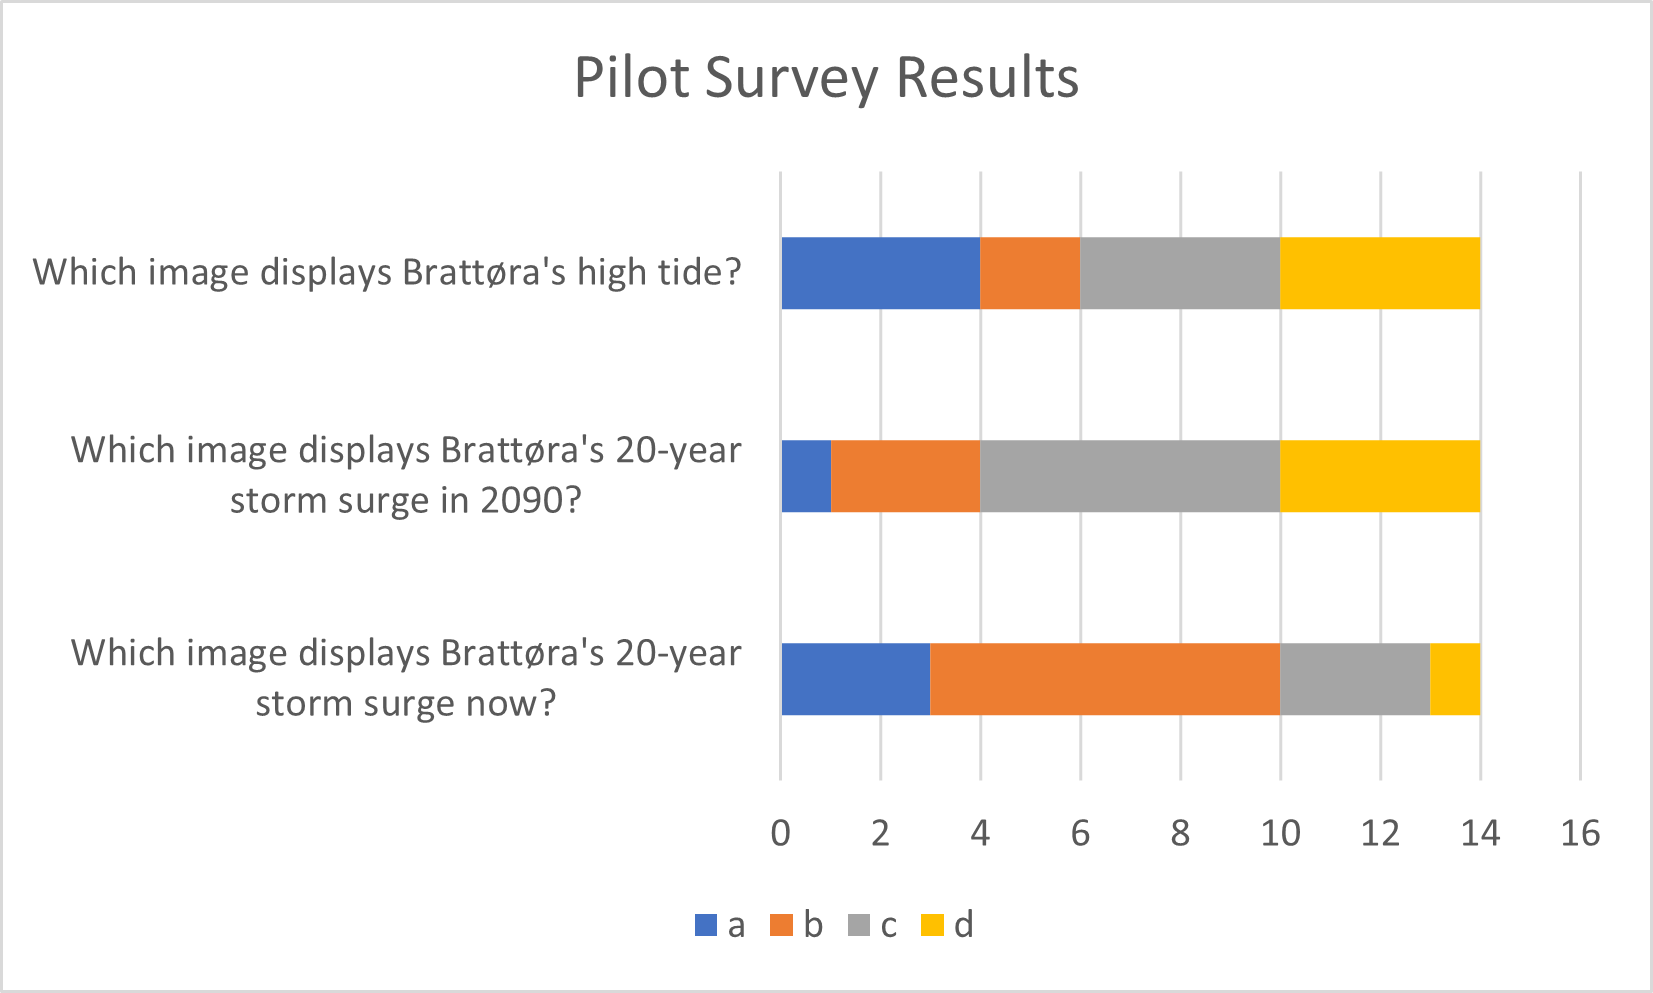
\includegraphics{fig_results/pilot-survey-results.png}
    \caption{Pilot Survey Results - The answers which matches the model \cite{kartverket_se_2021} were always B, here coloured orange. This was done for ease of speedy analysis and discussion after survey completion.  As can be seen the majority chose answer B for question "which image display's Brattøra's 20-year storm surge now". However for "Which image display's Brattøra's 20-year storm surge in 2090?" the majority chose C, with D the next popular answer. for "Which image displays Brattøra's high tide?" the responses were very spread, with B being the least popular, even though it matched the model from \cite{kartverket_se_2021}    }
    \label{fig:pilot_survey_results}
\end{figure}

As can be seen the pilot survey subjects did not easily get the correct answers for sea level extremes in Trondheim. The answer which corresponds with the model from \cite{kartverket_se_2020}, for each of the questions is B, which is represented in orange in figure 5.1 above. The responses for the question of the high tide were very spread, with the answer corresponding with the model from \cite{kartverket_se_2020}, being the least popular.  Answer C was the most popular when responding about the 20 year storm surge in 2090. In contrast the majority of subjects did chose the answer which corresponds with the model when being asked about where the current 20 year storm surge is. The lack of answers which corresponded with models was of concern with a group who appeared to have high awareness of sea level extremes, so a focus group was run. 
\paragraph{}


\subsection{Focus Group Results}
 The results from the focus group was that the maps were too similar, especially when using smart phones. It was too difficult to tell the maps apart due to the relatively small changes. This was particularly the case for the question about the high tide. Furthermore, several participants highlighted that they did not think of sea level extremes in terms of area flooded, but solely in terms of changing height. This one dimensional view was highlighted as a limiting factor in the understanding of potential impacts. 
\paragraph{}

The focus group were shown the slide featured below - figure 5.2. They were then asked which visualisation would help them answer the questions set in the pilot survey.
\paragraph{}

\begin{figure}[h!]
    \centering
    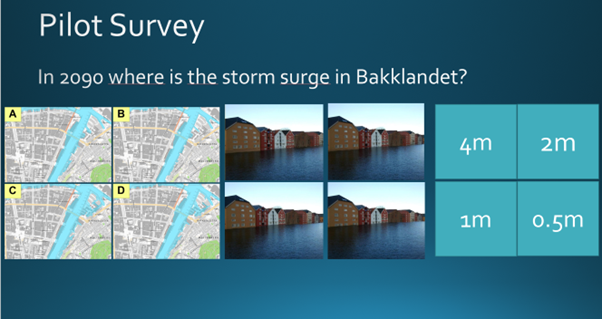
\includegraphics[width=1\textwidth]{fig_results/slide-pilot-survey.png}
    \caption{Slide shown to the focus group. The first image is how sea level extremes could be visualised using maps of the area. The second image is how sea level extremes could be visualised using photo editing of the waterline. The third image is how the sea level extremes could be visualised in a numeric way. This slide was used to spark discussion and allow for comparison.}
    \label{fig:slide}
\end{figure}

Several of the participants chose numeric value visualisation, but recognised that was likely due to their professional background. Those with a longer knowledge of Trondheim favoured the simulated sea level extremes pictures. This was also highlighted as the option with the highest emotional impact and the visualisation which caught the whole focus groups attention.

\paragraph{}

The results of the focus group and pilot survey were that this method was reasonable for determining awareness but that a combination of numerical and image based visualisation of sea level extremes would be used, rather than map based. This decision did loose the spatial aspect of communication, but allowed for greater emotional connection.

\section{Technological Systems}

Distinguishing technological and natural systems can be difficult in a landscape which has been actively shaped by its population for so long. The interaction between each of the systems of which the interplay results in the projected resilience is significant. For Trondheim the location of infrastructure including buildings and roads is the primary focus of the technological system which impacts resilience to sea level extremes. How this infrastructure is built is of course of great importance to whether a speedy return to normality is possible after a sea level extreme event. Norway has strict building regulations, with further rules about infrastructure in vulnerable locations \cite{direktoratet_for_byggkvalitet_direktoratet_nodate}. Yet even perfectly designed infrastructure will still be impacted if flooded. Impacts range from the obvious  prevention of use during flooding, to post event clean up and the wear and damage which can occur from sea level extreme events.
\paragraph{}
The table below displays the number of building which are likely to be impacted during different sea level extremes in Trondheim. This is modelled by \cite{kartverket_se_2021} and was the base of later water level simulations as used in this project. Importantly this modelling is more localised than previous models of sea level extremes in Norway.

\begin{table}[h]
    \centering
    \begin{tabular}{|l|l|l|l|l|}
    \hline
        water level & no. buildings  & ~ & ~ & ~ \\ \hline
        ~ & private & private & public  & critical  \\ \newline
        ~ & buildings & businesses & buildings & buildings \\ \hline        
        20 years return height now & 160 & 77 & 10 & 0 \\ \hline
        200 years return height now & 214 & 87 & 10 & 0 \\ \hline
        1000 years return height now & 242 & 104 & 14 & 0 \\ \hline
        Flooded 2090 & 66 & 51 & 8 & 0 \\ \hline
        20-years return height 2090 -& 264 & 119 & 17 & 1 \\ \hline
        200-years return height  2090 & 308 & 136 & 24 & 1 \\ \hline
        1000-years return height  2090 & 332 & 148 & 26 & 1 \\ \hline
        1m sea level rise & 127 & 64 & 9 & 0 \\ \hline
        2m sea level rise & 343 & 155 & 29 & 1 \\ \hline
        3m sea level rise & 584 & 285 & 55 & 3 \\ \hline
        4m sea level rise & 752 & 335 & 70 & 5 \\ \hline
        5m sea level rise & 1023 & 402 & 77 & 8 \\ \hline
    \end{tabular}
    \caption{Impact of Sea Level Extremes, the Number of Buildings Flooded from \cite{kartverket_se_2021} - The major contrast between current 20 year storm surge and the 2090, 20 year storm surge is that at the water level is high enough to flood a critical. Flooding of a critical building would also occur at 2m sea level rise.}
    \label{building-impact-sle}
\end{table}


Table 4.1 shows that there is currently some risk from sea level extremes. The current 20 year return height is projected to cause the flooding of 247 buildings. However it is worth noting that no critical buildings are predicted to flood even with the 1000 year return height. This is in contrast to the 20 year return height in 2090, which is projected to cause the flooding of one critical building.

Norway's economy and residency patterns are very dependent on activities along the coast\cite{aunan_strong_2008}, as can be seen above Trondheim also has some dependency on coastal activities. The information here will be used to discuss Trondheim's technological resilience to sea level extremes in the discussion. 


\section{Natural Systems}
Natural system focused upon in this section is the changing water levels expected with different see level extremes. 

\subsection{Visual Simulation Sea Level Extremes}
The figures below display the simulated sea level extremes created for this project based off \cite{kartverket_se_2020}.

\begin{figure}[h!]
    \centering
    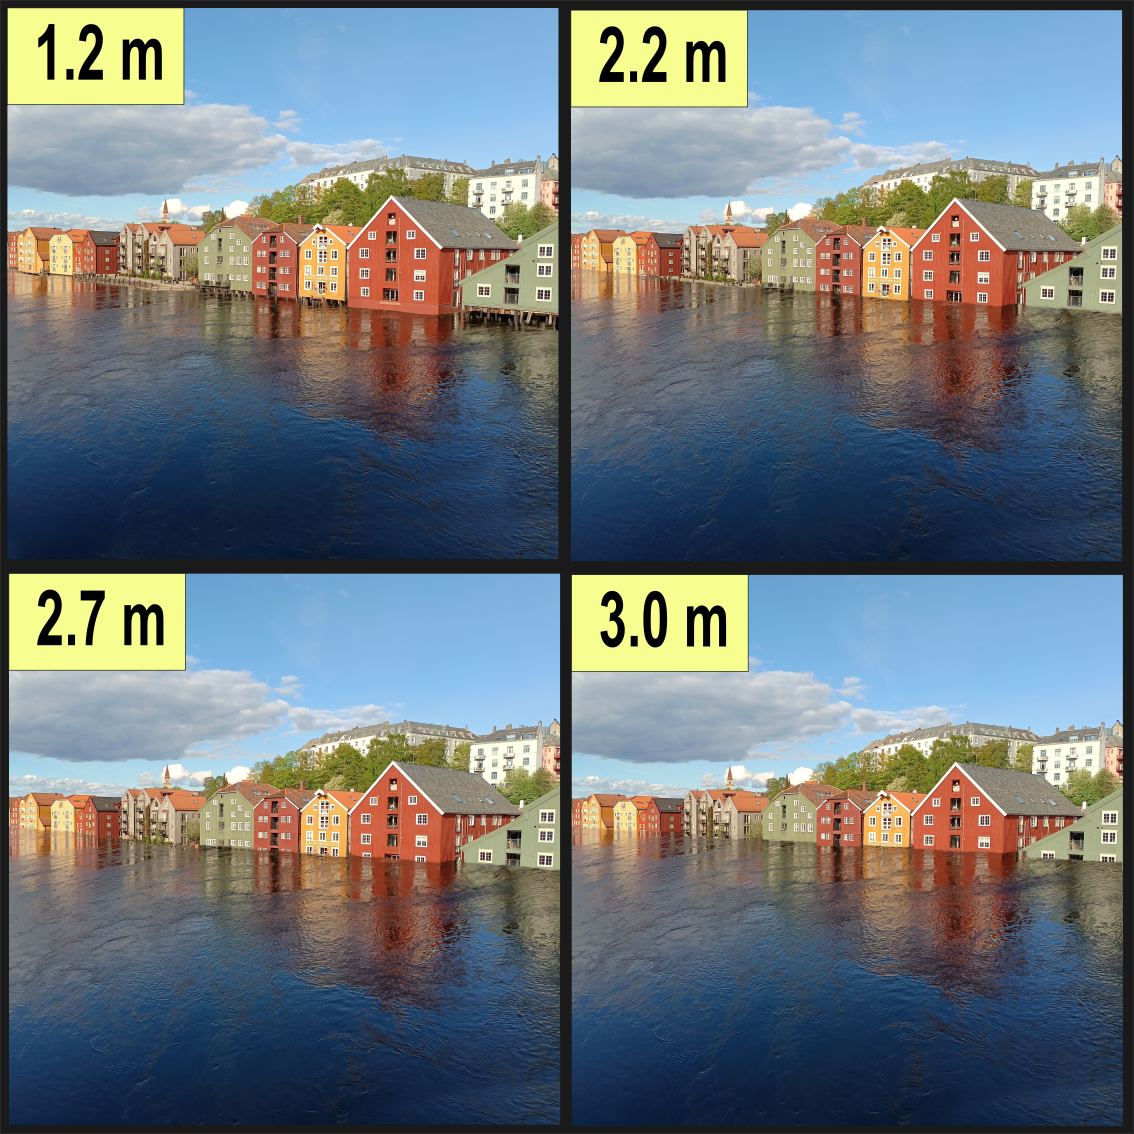
\includegraphics[width=10cm]{fig_sle/nidelva 2090 q.png}
    \caption{Simulated Sea Level Extremes for Nidelva research site - These were created using \cite{kartverket_se_2021} and \cite{stormflo_database_stormflo_2021}. }
    \label{fig:SLE-nidelva}
\end{figure}

\begin{figure}[h!]
    \centering
    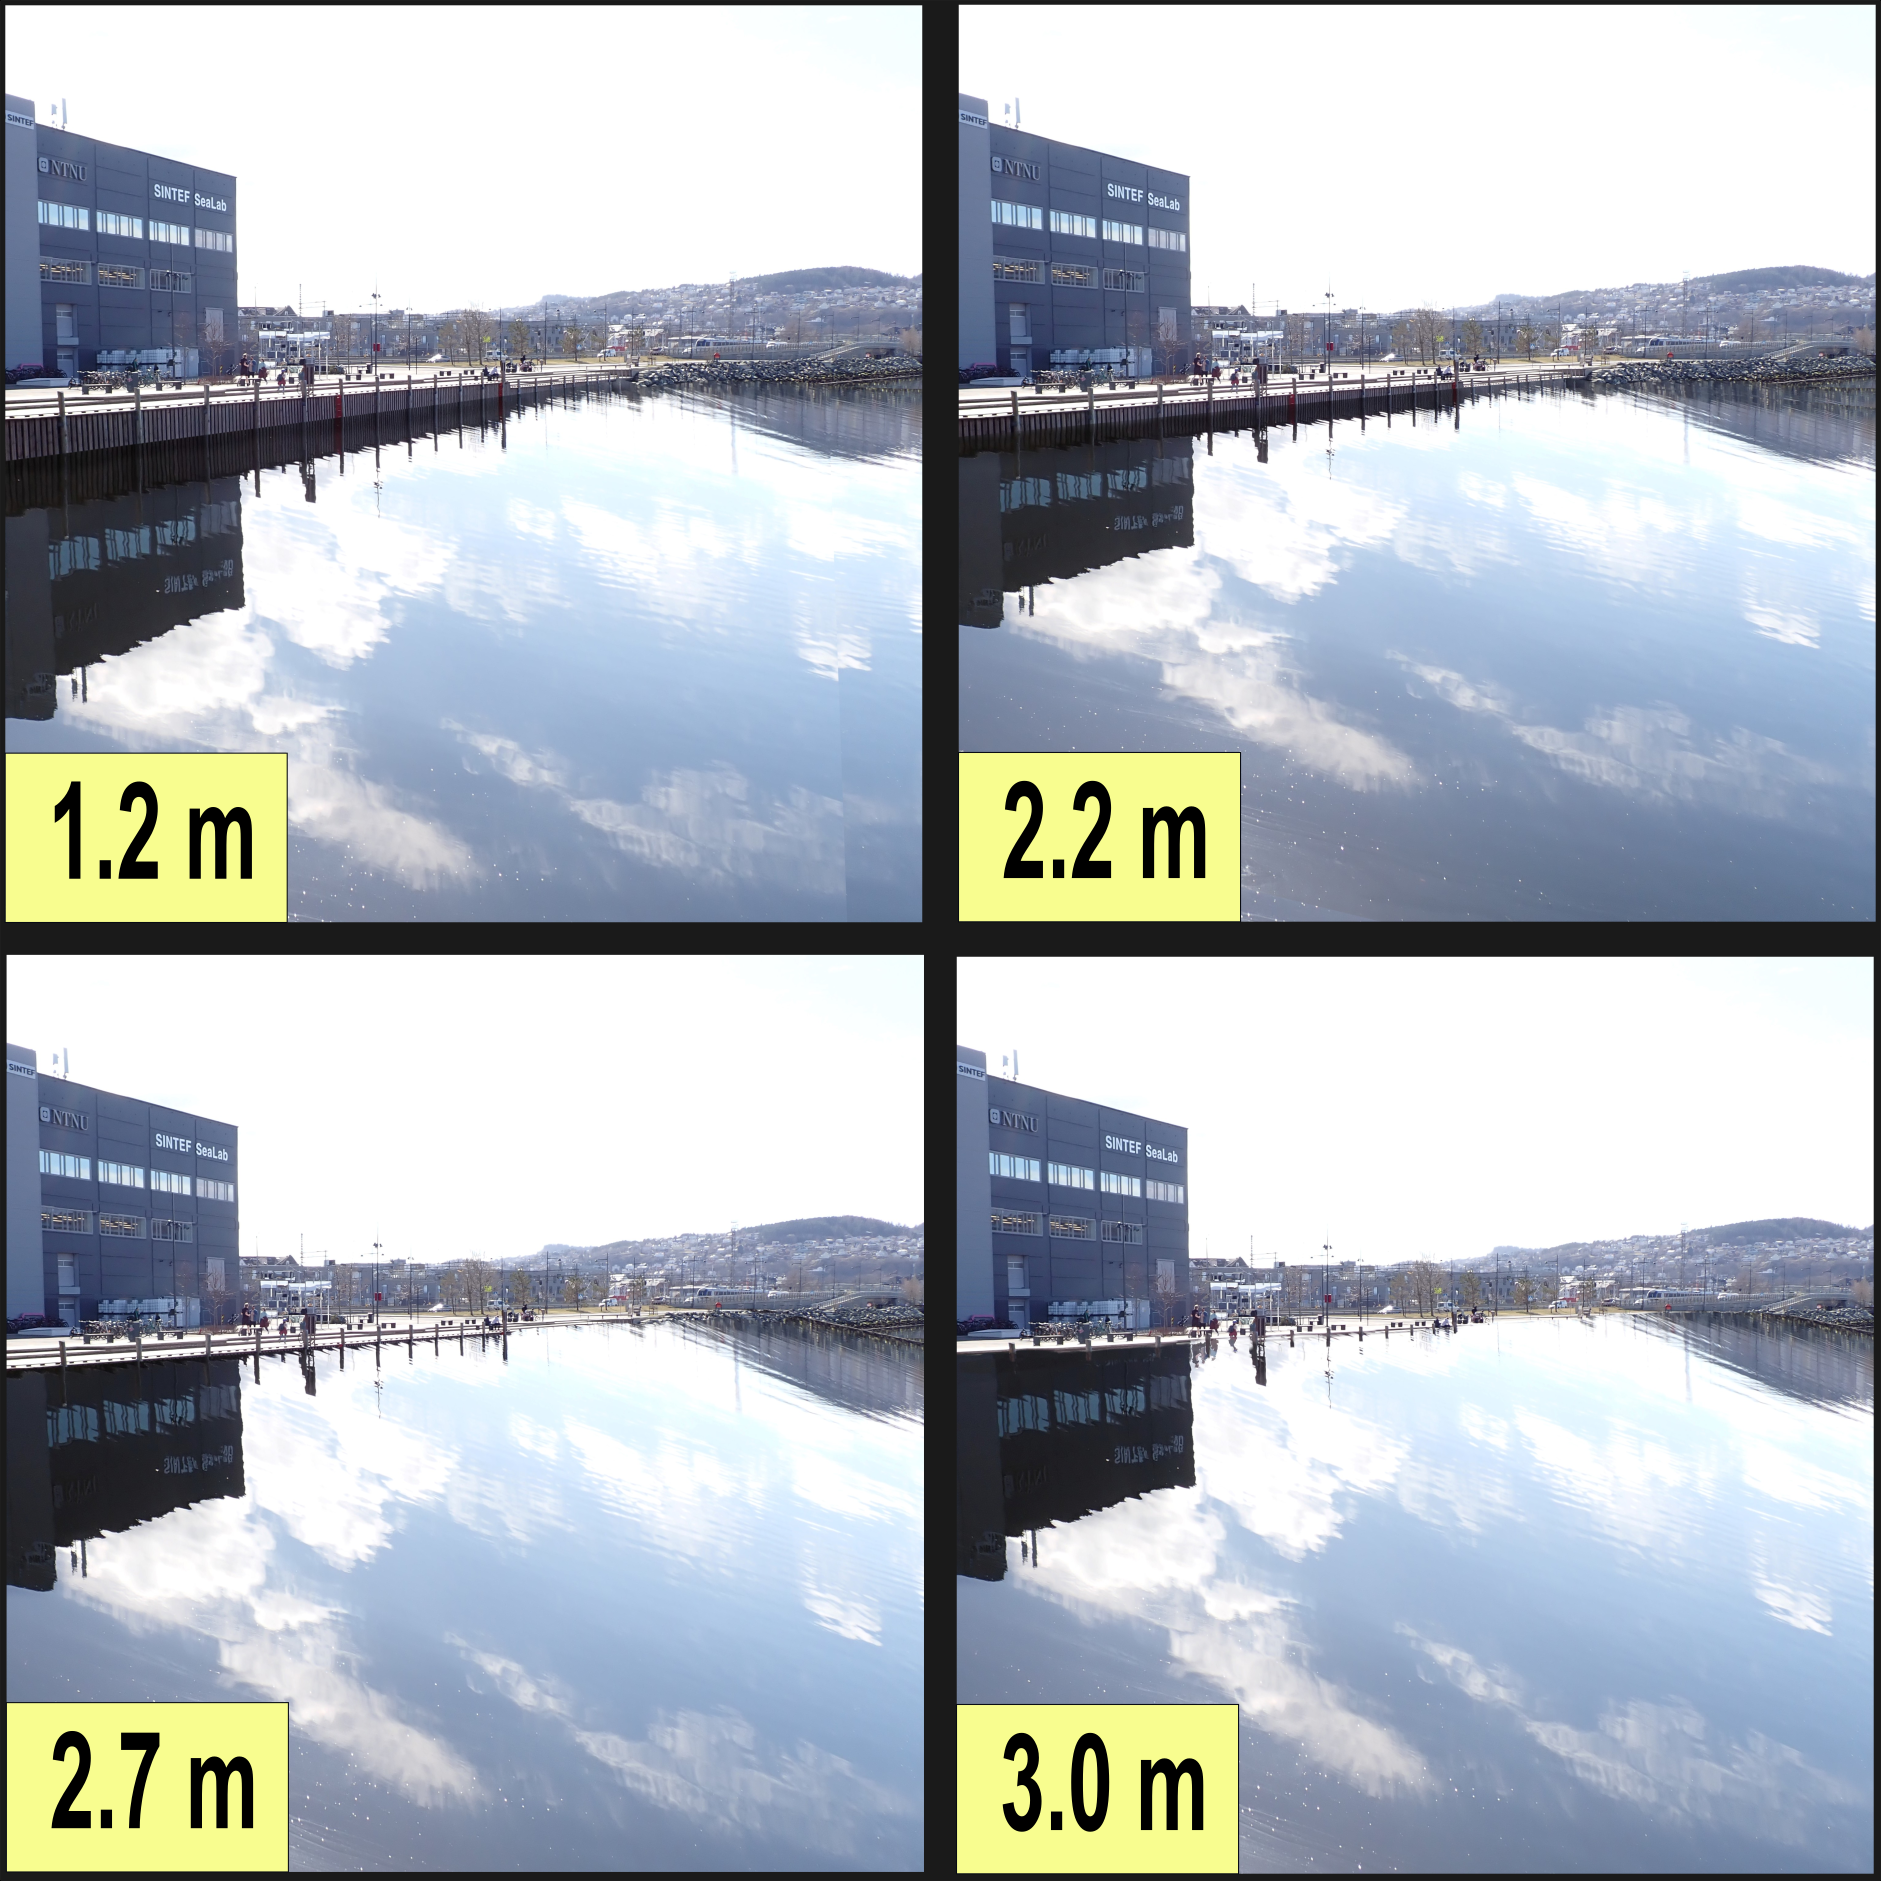
\includegraphics[width=10cm]{fig_sle/brattora 2090 q.png}
    \caption{Simulated Sea Level Extremes for Brattøra research site - These were created using \cite{kartverket_se_2021} and \cite{stormflo_database_stormflo_2021}. }
    \label{fig:SLE-brattora}
\end{figure}

\begin{figure}[h!]
    \centering
    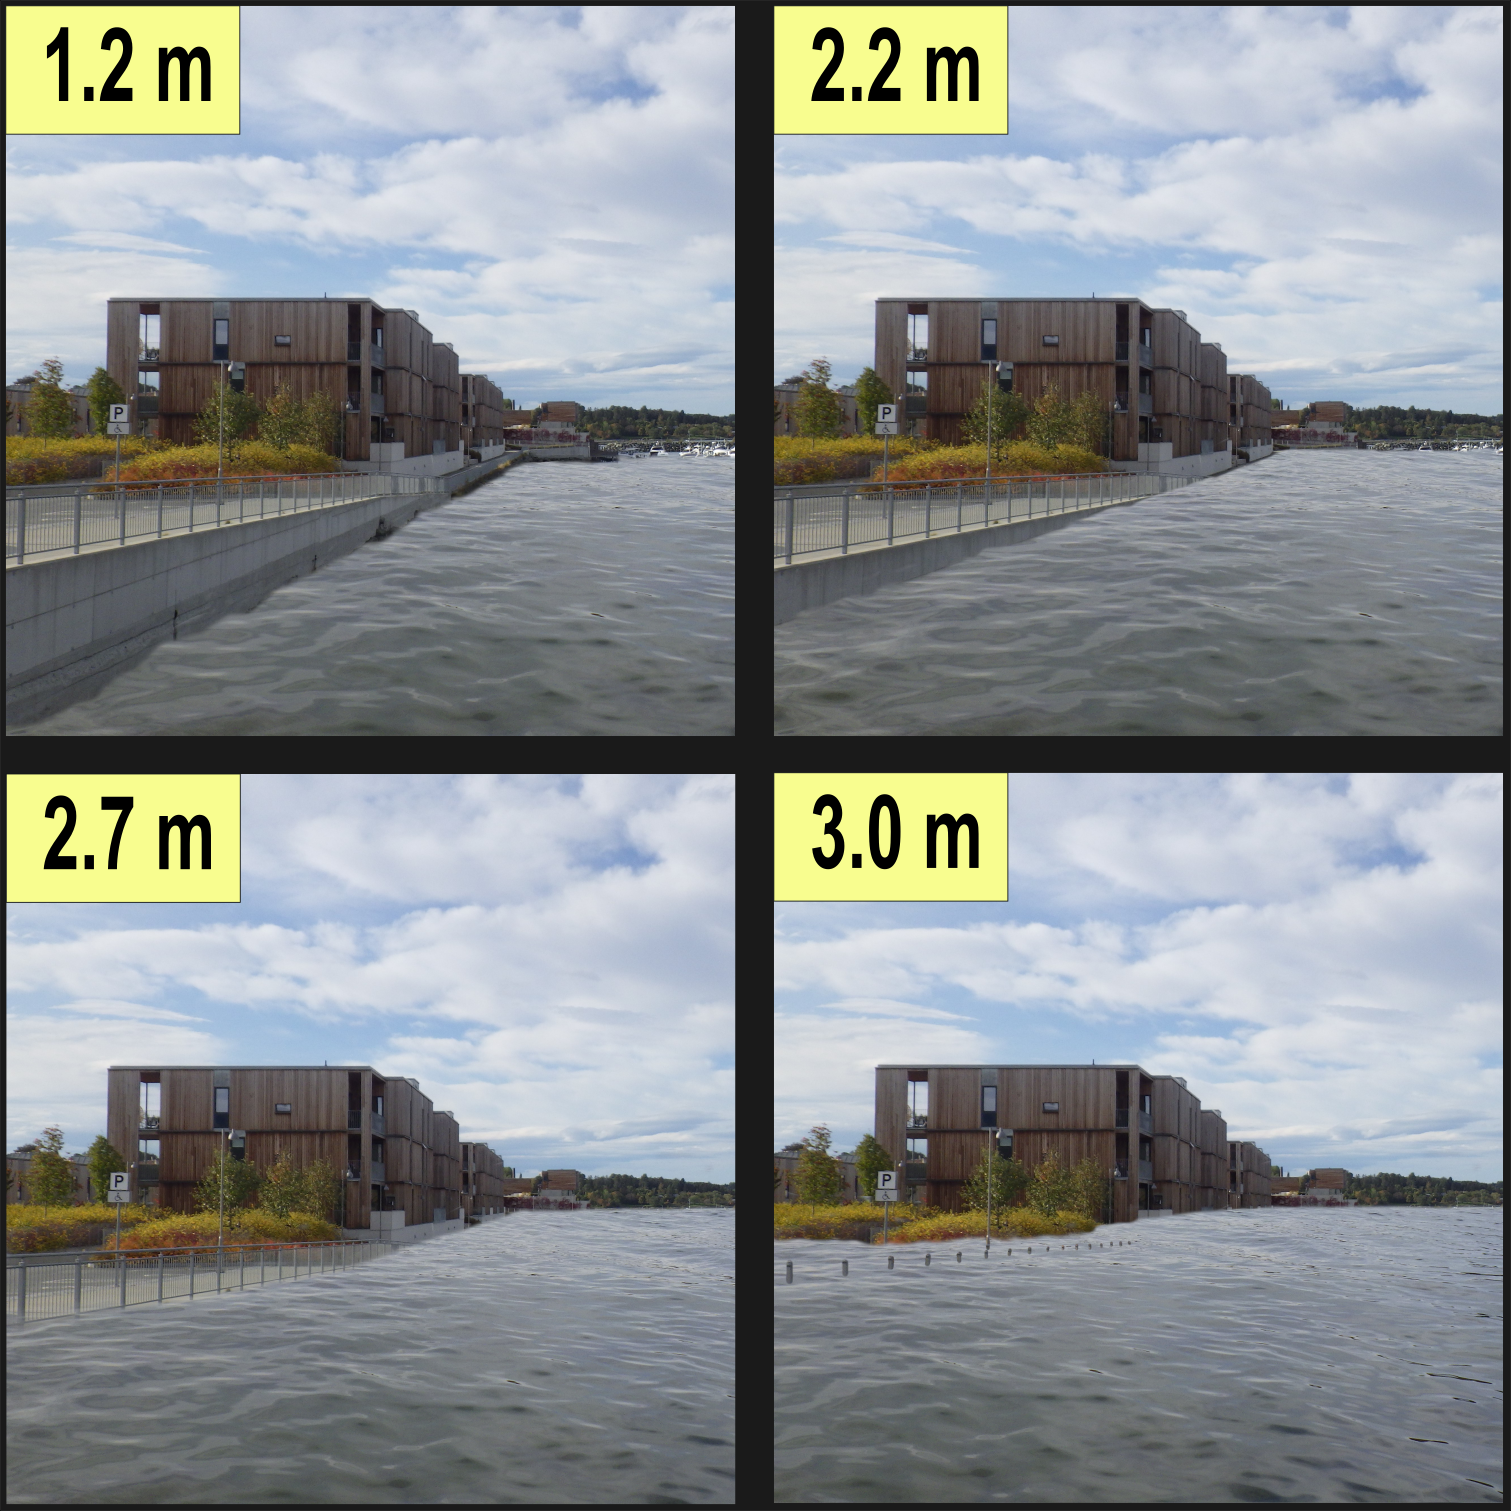
\includegraphics[width=10cm]{fig_sle/grillstad 2090 q.png}
    \caption{Simulated Sea Level Extremes for Grillstad research site - These were created using \cite{kartverket_se_2021} and \cite{stormflo_database_stormflo_2021}. }
    \label{fig:SLE-grillstad}
\end{figure}

\begin{figure}[h!]
    \centering
    \includegraphics[width=10cm]{fig_sle/illsvika 2090 q.png}
    \caption{Simulated Sea Level Extremes for Skansen research site - These were created using \cite{kartverket_se_2021} and \cite{stormflo_database_stormflo_2021}. }
    \label{fig:sle-skansen}
\end{figure}


Figure 5.3, 5.4, 5.5 and 5.6 display the sea level extremes simulated for this project based off \cite{kartverket_se_2020}. The differing heights represent different potential events. 1.2m is a very likely event as this is the height associated with the spring high tide for each of the research sites. 2.2m is a lot less likely as it represents the water level height associated with the current 20 year storm surge. While a water level of 2.7m is projected for the 20 year storm surge in 2090. Finally the 1000 year storm surge in 2090 is represented by 3.0m as seen in the bottom right of each of the figures.
\paragraph{}
The changing sea level extremes are not that significant in terms of height. Due to the geological setting discussed in the background the natural systems resilience is high. However, the figures above also display how this interplay's with technological and social system resilience, changing the ability to quickly return to normality depending on the water level. 

\subsection{Sea Level Extremes Maps}
i.e. can do the same as above with maps if desired 




\section{Social Systems}

This chapter focuses on the results gained from the survey conducted to determine social resilience to sea level extremes in Trondheim.  It also includes the results from Kruskal Wallis Rank Sum Tests and Shapiro Tests. Each of the results gained from the survey questions is displayed in a graph. These results will be discussed to determine Social Systems Resilience to Sea Level Extremes in the discussion. The tables and graphs below make reference to  the questions in the survey these results were gained from. For the full survey in either Norwegian or English please consult the appendix. Reference in text is only made to the English questions for ease of readability. 



\subsection{Place and language}
There were 153 subjects who conducted the survey. The survey was split into 8 subsurveys which the sunjects could chose from. Surveys were conducted focusing on Skansen, Grillsta, Brattøra and Nidel
\begin{table}[h]
    \centering
    \begin{tabular}{|l|l|}
    \hline
    Place  & No. Subjects  \\ \hline
      Skansen   & 29    \\ \hline
      Nidelva & 57      \\ \hline
      Grillstad & 37       \\ \hline
      Brattøra & 30     \\ \hline
      Total & 153   \\ \hline
     \end{tabular}
    \caption{Place subjects chose to Answer on. The most popular place to Respond was Nidelva with 57 response representing 37 percent of responses. Next popular was Grillstad with 37 responses and then Brattøra with 30 and Skansen with 29 respectively. The reasonable spread of response does allow for comparison}
    \label{tab:place}
\end{table}
\paragraph{}

As can be seen in the table above the most popular place for responses was Nidelva. This is the most central of the locations and has  the greatest daily throughput of people. It also includes perhaps the most iconic views of Trondheim. Next popular was Grillstad, perhaps due to the recognition by residents that the area could be severely influenced by flooding from sea level extremes. Skansen and Brattøra are the next most responded to, both of these locations have significant commercial ventures. Brattøra in particular is dominated not by residency but by offices and industry. Perhaps the conduction of this survey in Summer decreased the number of responses due to the lack of office workers. 
Almost evenly split for each location was whether the survey was completed in Norwegian or English. English surveys had 66 response, while the Norwegian survey had 87 responses.  

\subsection{Interest Level in Sea Level Extremes}
Awareness as a facet of local knowledge was the searched for variable within this project. An interesting comparison is level of interest against awareness. There is the assumption that high or professional interest in sea level extremes is associated with higher levels of awareness of the risk. 
\begin{figure}[h]
    \centering
    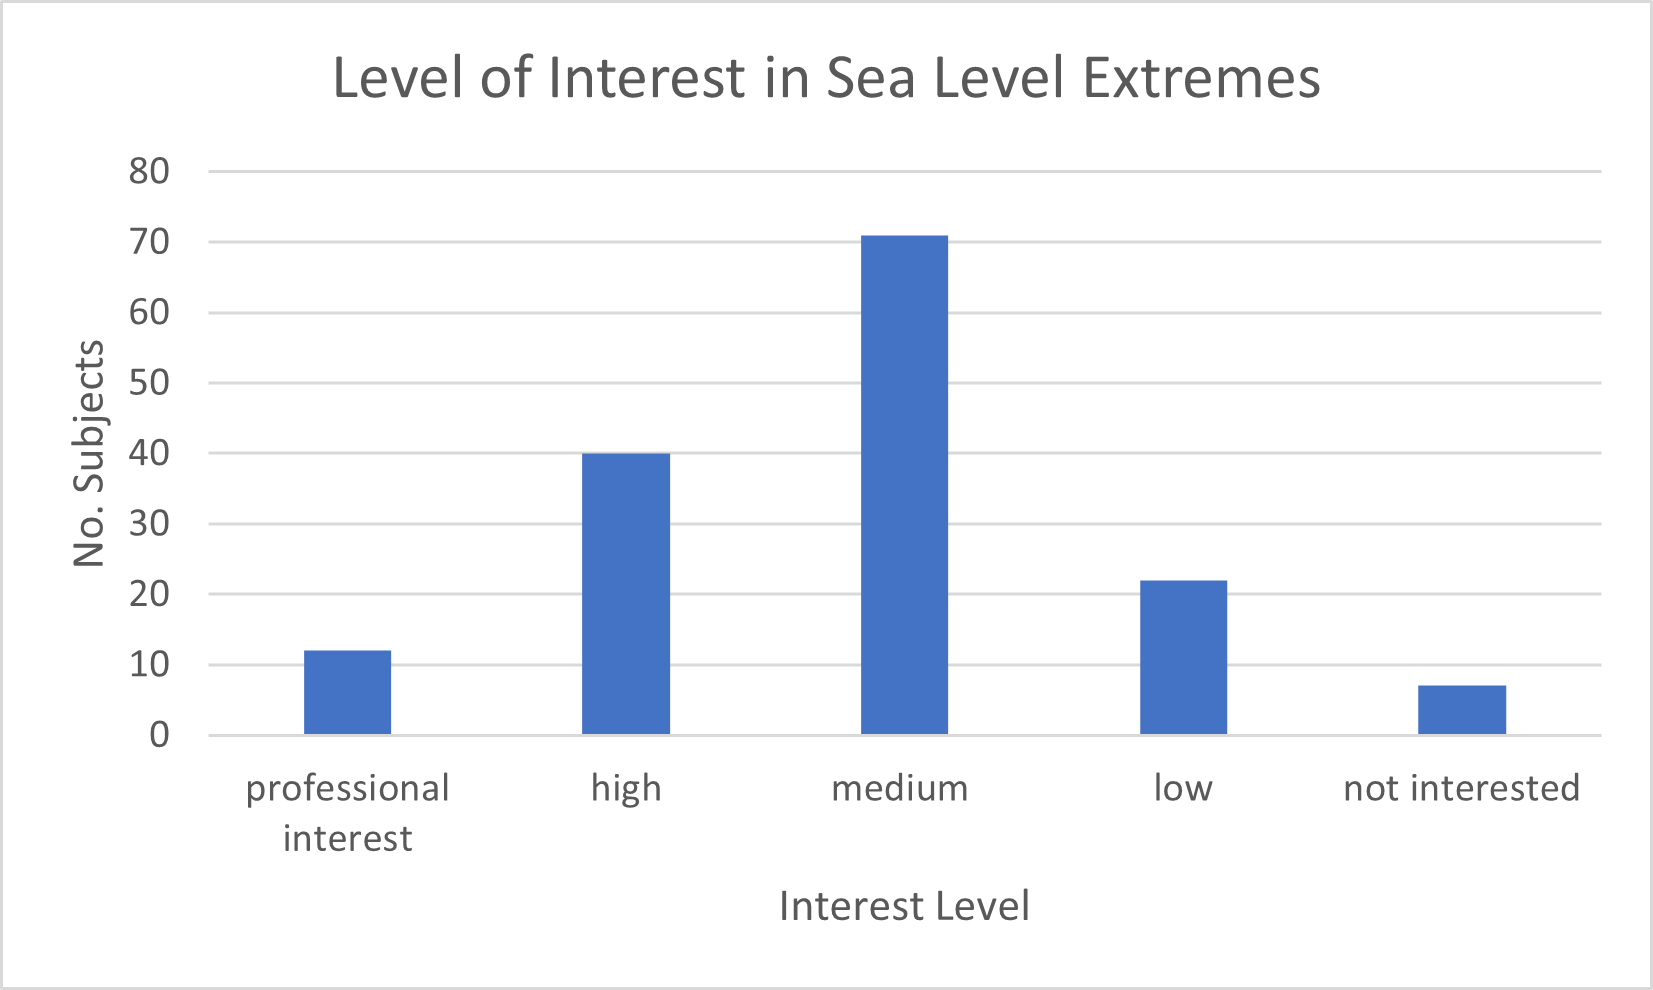
\includegraphics{fig_results/interest-level.png}
    \caption{Interest Level in Sea Level Extremes}
    \label{fig:my_label}
\end{figure}
\paragraph{}
words words words

\begin{figure}[h]
    \centering
    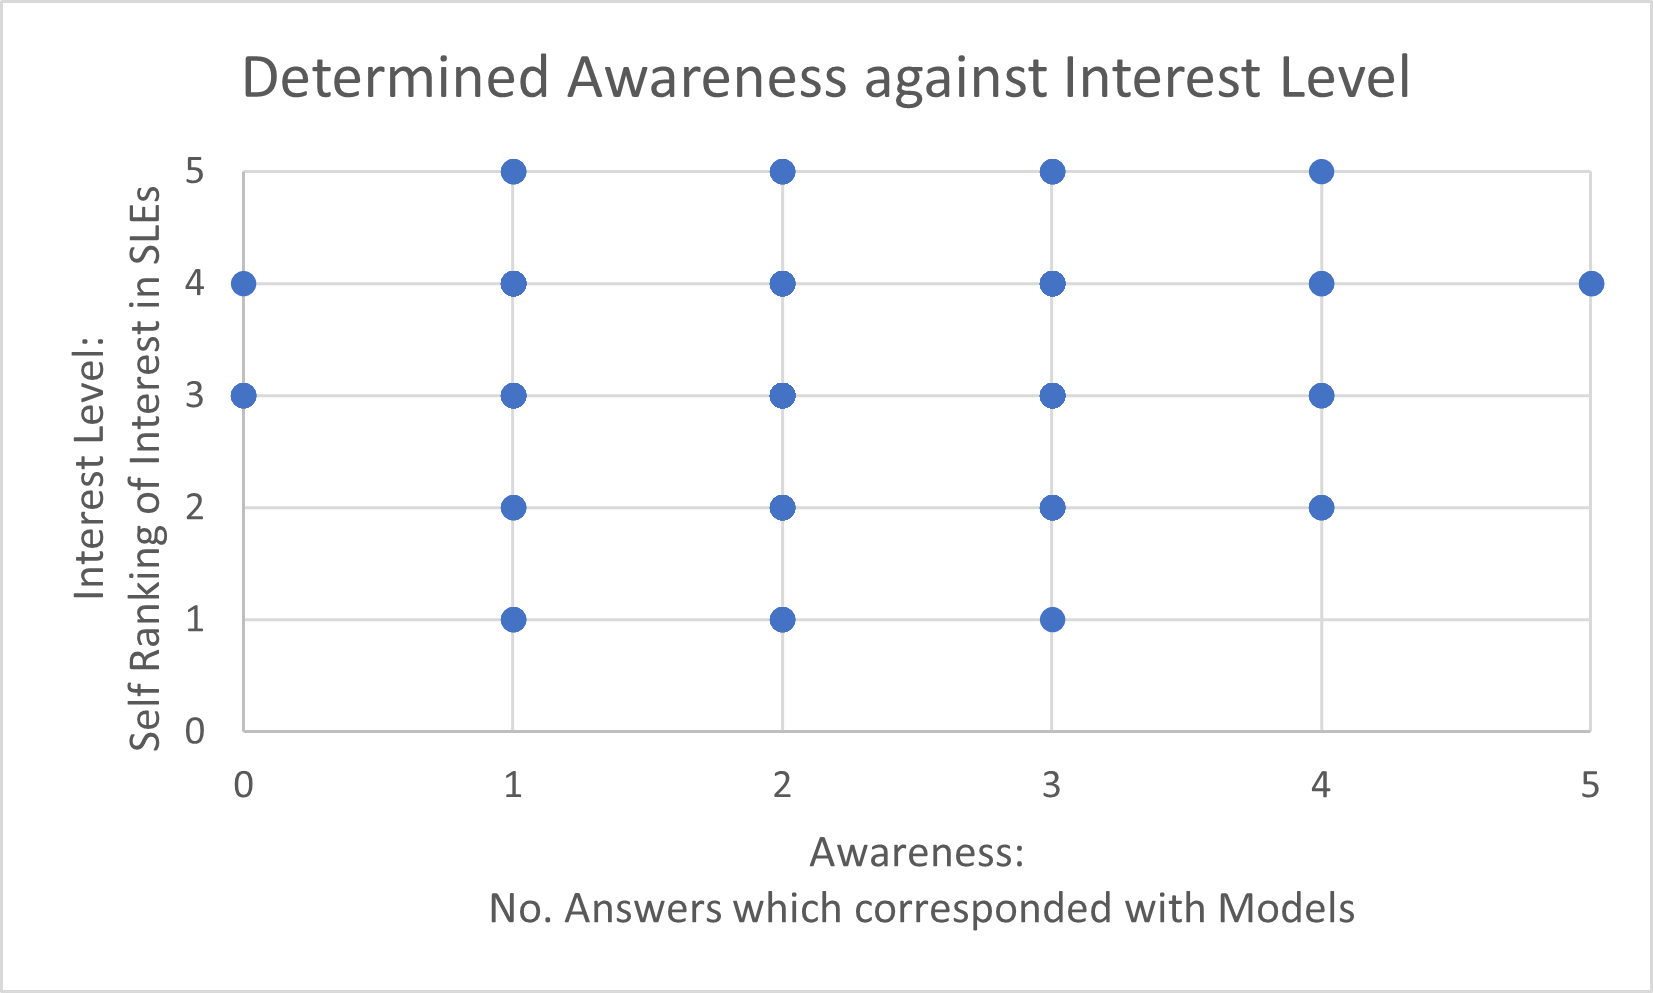
\includegraphics{fig_results/aware_vs_interest.png}
    \caption{Determined Awareness Against Interest Level}
    \label{fig:aware_vs_interest}
\end{figure}[]
\paragraph{}

There is no linearity between this determination of awareness and self determined interest level. This raised questions about the assumption of resilience due to the prescence of professionals within a community. However there is serious limitations on this result as there were no marine workers included in the surveys subjects.


\subsection{Memory of Sea Level Extremes}

\begin{figure}[h]
    \centering
    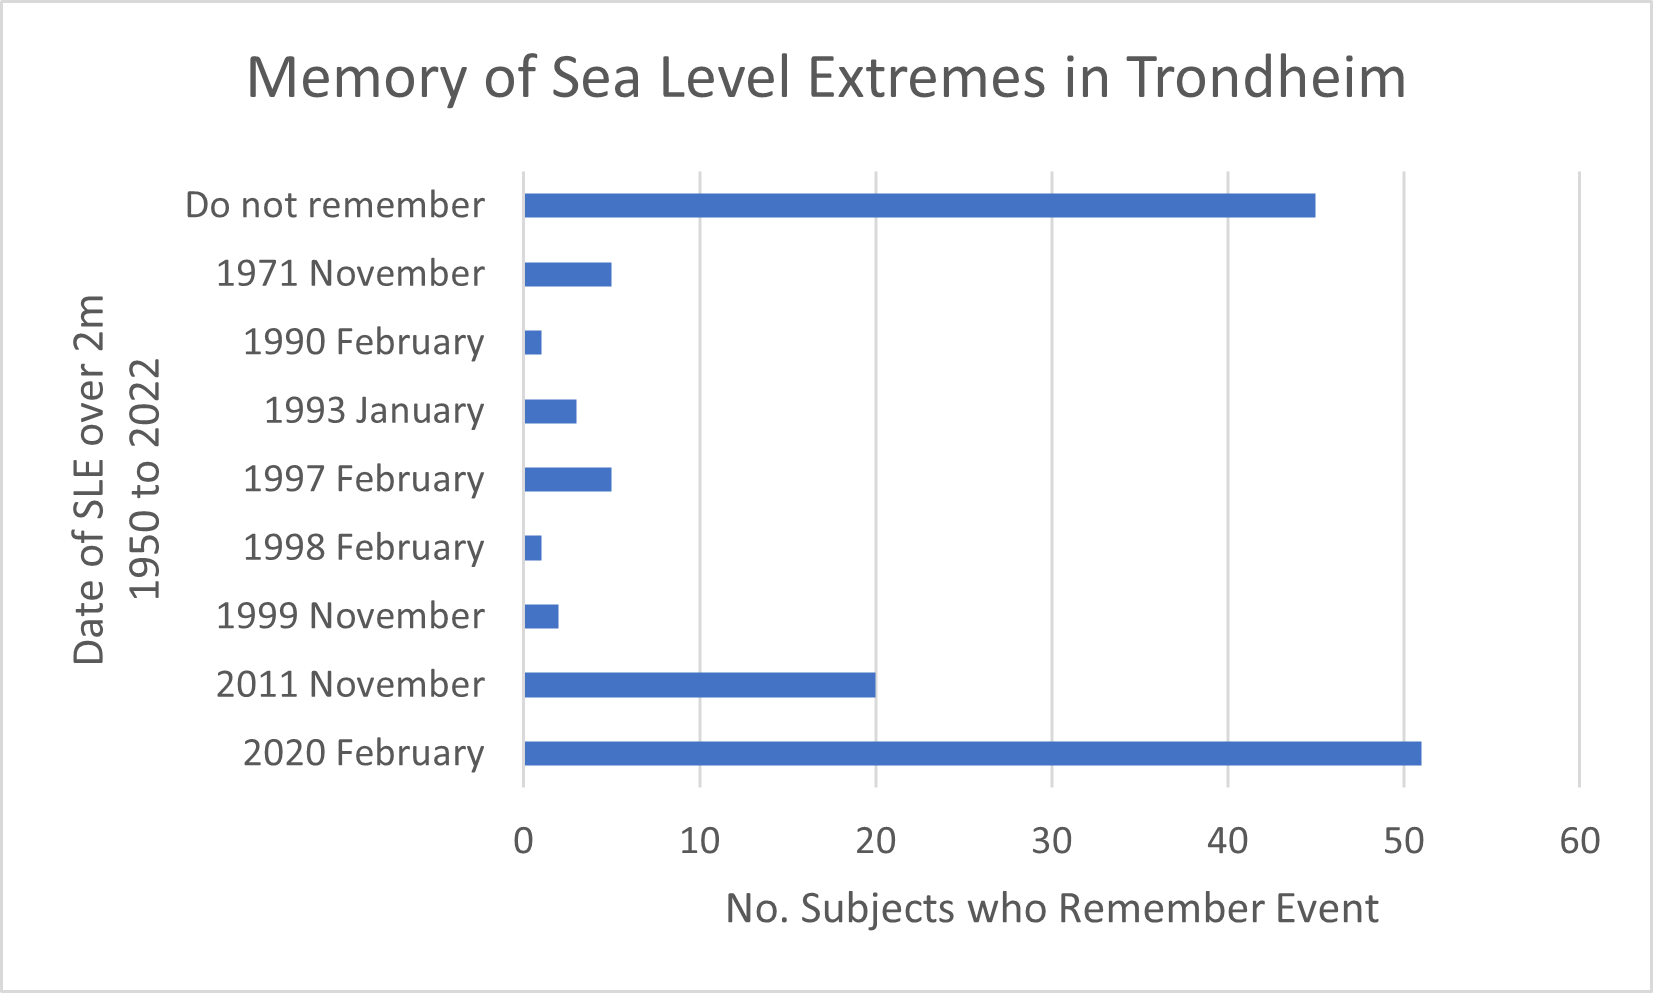
\includegraphics{fig_results/memory-sle.png}
    \caption{Memory of Sea Level Extremes}
    \label{fig:my_label}
\end{figure}
\paragraph{}


As can be seen in the figure above this is a very skewed factor. T Value 0 is the most common and displays the number of subjects with no memory of sea level extremes in Trondheim. Each other number indicates the number of sea level extreme events (water level higher than 2m) the subject remembered occurring between 1950 and summer 2022. For the full list of potential events please consults the relevant question in the appendix. Relatively few subjects remembered sea level extremes. The lack of memory is very interesting considering that length of knowledge for the majority included two sea level extreme events as can be seen in the figure below. 

\begin{figure}[h!]
    \centering
    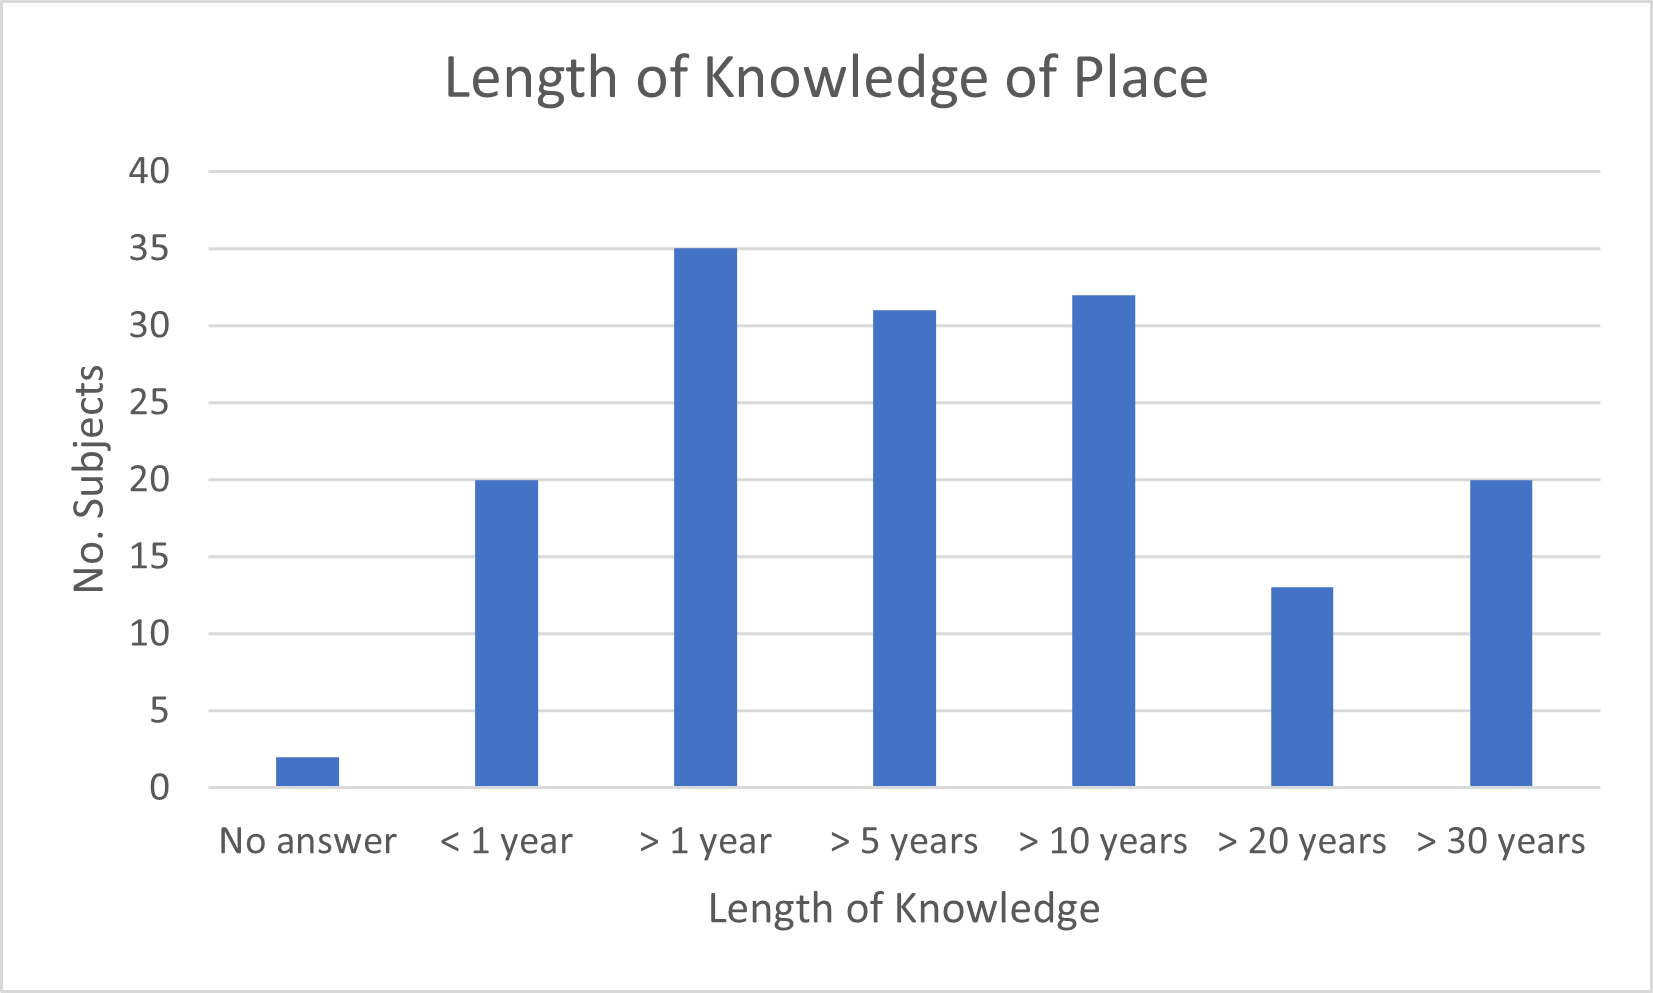
\includegraphics{fig_results/long_know.png}
    \caption{Length of Knowledge of Subjects. 96 subjects had a length of knowledge about the place greater than 5 years. 35 subjects had length of knowledge less than 5 years, but more than 1. Only 20 respondents had a length of knowledge under 1 year}
    \label{fig:long_know}
\end{figure}[]


\subsection{Level of Interest in Sea Awareness}

\begin{figure}[h]
    \centering
    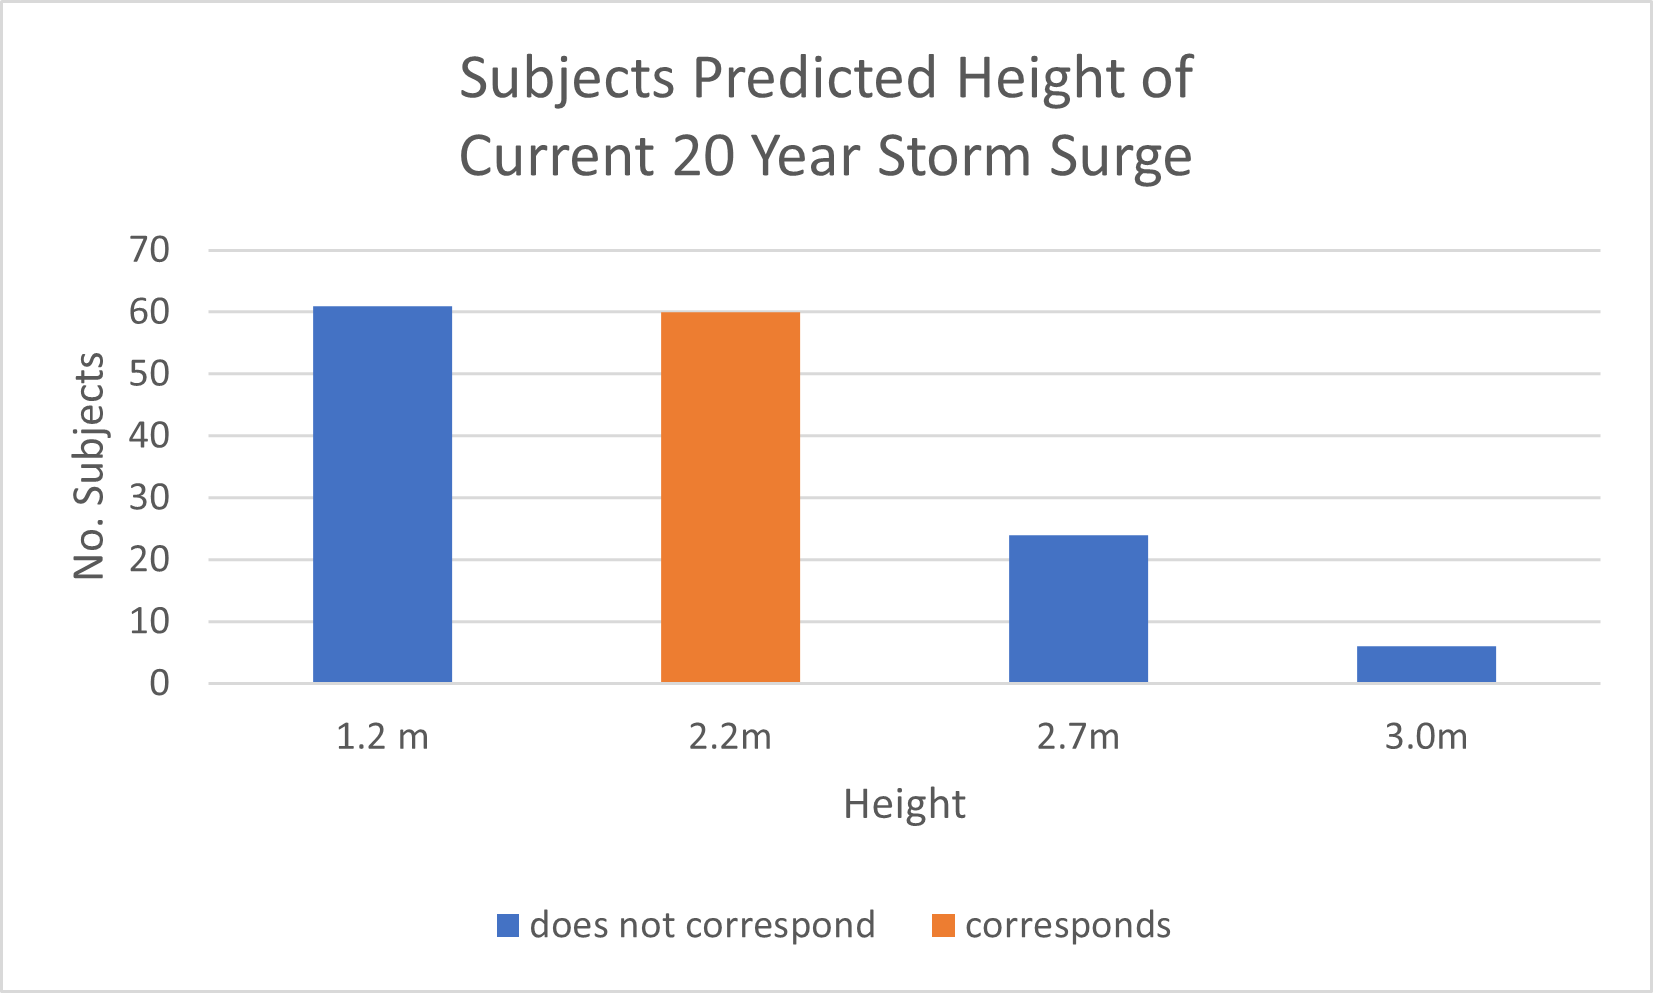
\includegraphics{fig_results/2022-20yrss-answer.png}
    \caption{Level of Interest in Sea Level Extremes}
    \label{fig:my_label}
\end{figure}
\paragraph{}
words word words



\subsection{Information Access about Climate and Place}

\begin{center}
\begin{table}[h]
    \centering
    \begin{tabular}{|l|l|l|l|l|l|l|}
    \hline
        Factor name & mean & Std Dev. & min & max & range & skew  \\ \hline
        
      Sum of Information Access & 3.50 & 1.72 & 0 & 8 & 8 & 0.24  \\ \hline
        Personal Observation  & 0.45 & 0.50 & 0 & 1 & 1 & 0.20 \\ \hline
        Family & 0.18 & 0.38 & 0 & 1 & 1 & 1.68  \\ \hline
        Friends & 0.23 & 0.42 & 0 & 1 & 1 & 1.28  \\ \hline
        Newspapers & 0.72 & 0.45 & 0 & 1 & 1 & -0.96 \\ \hline
        TV & 0.46 & 0.50 & 0 & 1 & 1 & 0.14 \\ \hline
        Social Media & 0.63 & 0.48 & 0 & 1 & 1 & -0.55 \\ \hline
        Membership of Organisations & 0.14 & 0.35 & 0 & 1 & 1 & 2.09 \\ \hline
        Reviewed Publications\_sci & 0.39 & 0.49 & 0 & 1 & 1 & 0.44 \\ \hline
        Formal Education & 0.29 & 0.46 & 0 & 1 & 1 & 0.89 \\ \hline
        
         \end{tabular}
    \caption{Information about Climate Summary Statistics information access}
\label{table:summary_stats_info_access}
\end{table}
\end{center}

\begin{center}
\begin{table}[h]
    \centering
    \begin{tabular}{|l|l|l|l|l|l|l|}
    \hline
        variable name & mean & Std Dev. & min & max & range & skew  \\ \hline
        info\_place\_sum & 1.94 & 1.34 & 0 & 8 & 8 & 1.61 \\ \hline
        info\_place\_po & 0.73 & 0.45 & 0 & 1 & 1 & -1.00  \\ \hline
        info\_place\_family & 0.10 & 0.31 & 0 & 1 & 1 & 2.56 \\ \hline
        info\_place\_friend & 0.19 & 0.39 & 0 & 1 & 1 & 1.57  \\ \hline
        info\_place\_newspaper & 0.35 & 0.48 & 0 & 1 & 1 & 0.64  \\ \hline
        info\_place\_tv & 0.14 & 0.35 & 0 & 1 & 1 & 2.09 \\ \hline
        info\_place\_so\_me & 0.33 & 0.47 & 0 & 1 & 1 & 0.73  \\ \hline
        info\_place\_mem & 0.04 & 0.19 & 0 & 1 & 1 & 4.70 \\ \hline
        info\_place\_kommune & 0.07 & 0.26 & 0 & 1 & 1 & 3.28\\ \hline
                
         \end{tabular}
    \caption{Information about Place Summary Statistics information access}
\label{table:summary_stats_info_access}
\end{table}
\end{center}



\subsection{Community Membership}

\begin{figure}[h]
    \centering
    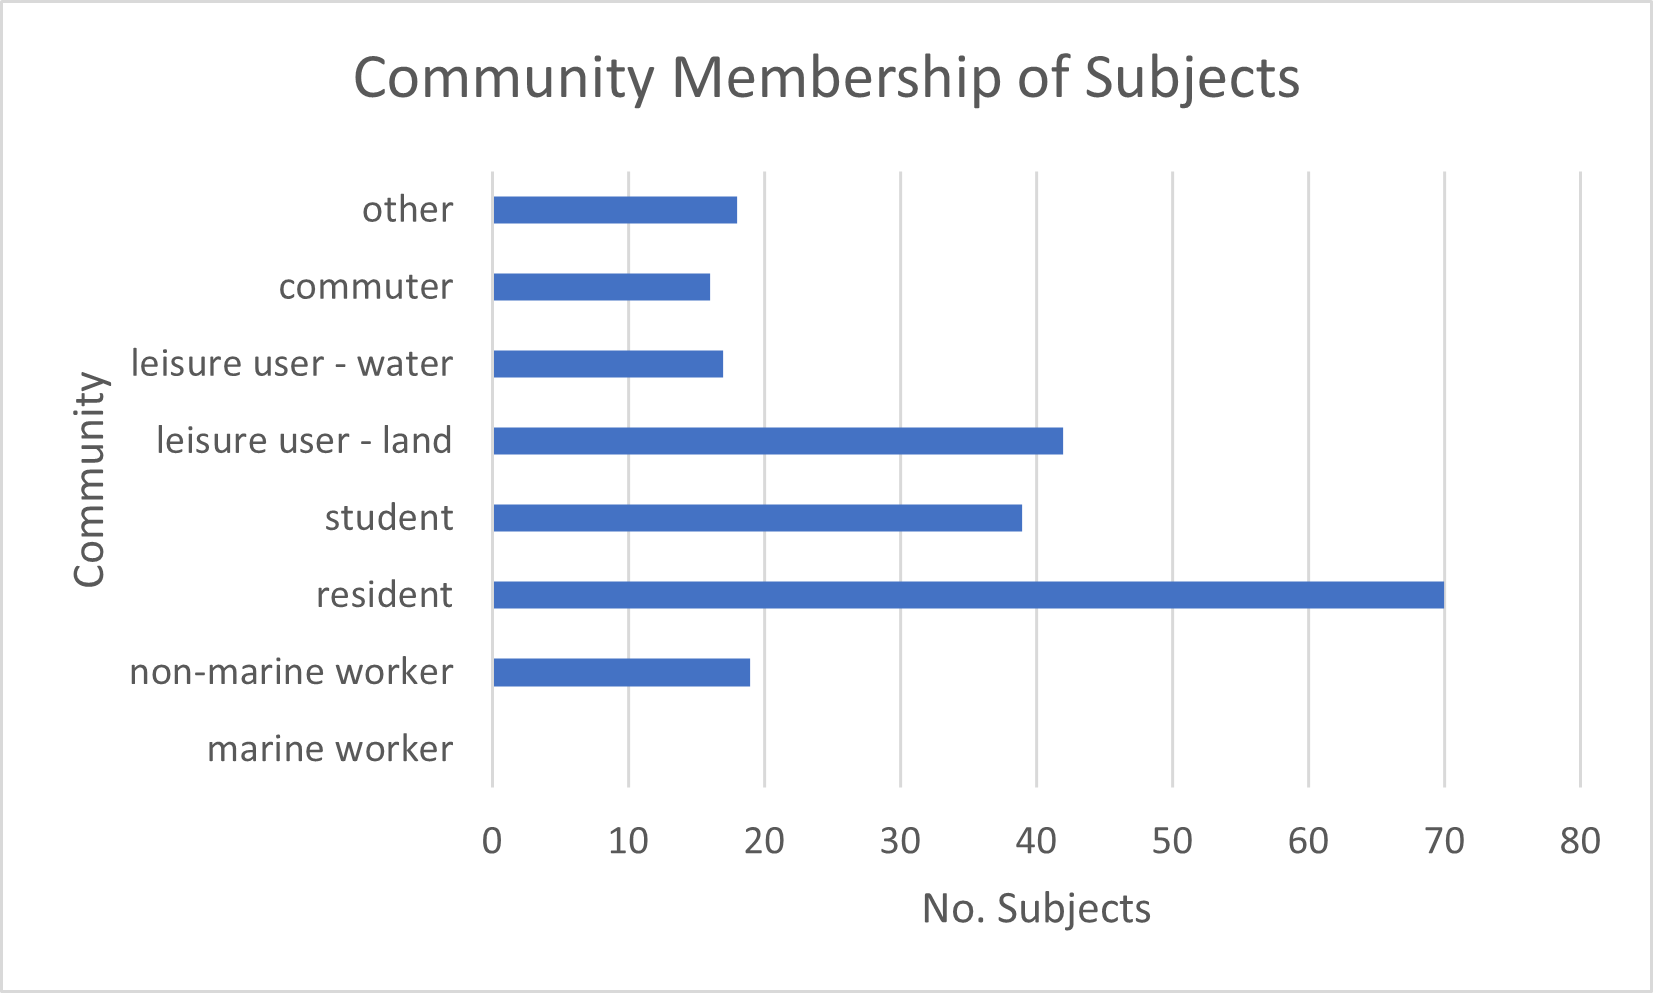
\includegraphics{fig_results/com-mem-horizontal.png}
    \caption{Membership of Communities}
    \label{fig:my_label}
\end{figure}
\paragraph{}
words words words 
\subsection{Access to Survey. }

\begin{figure}[h]
    \centering
    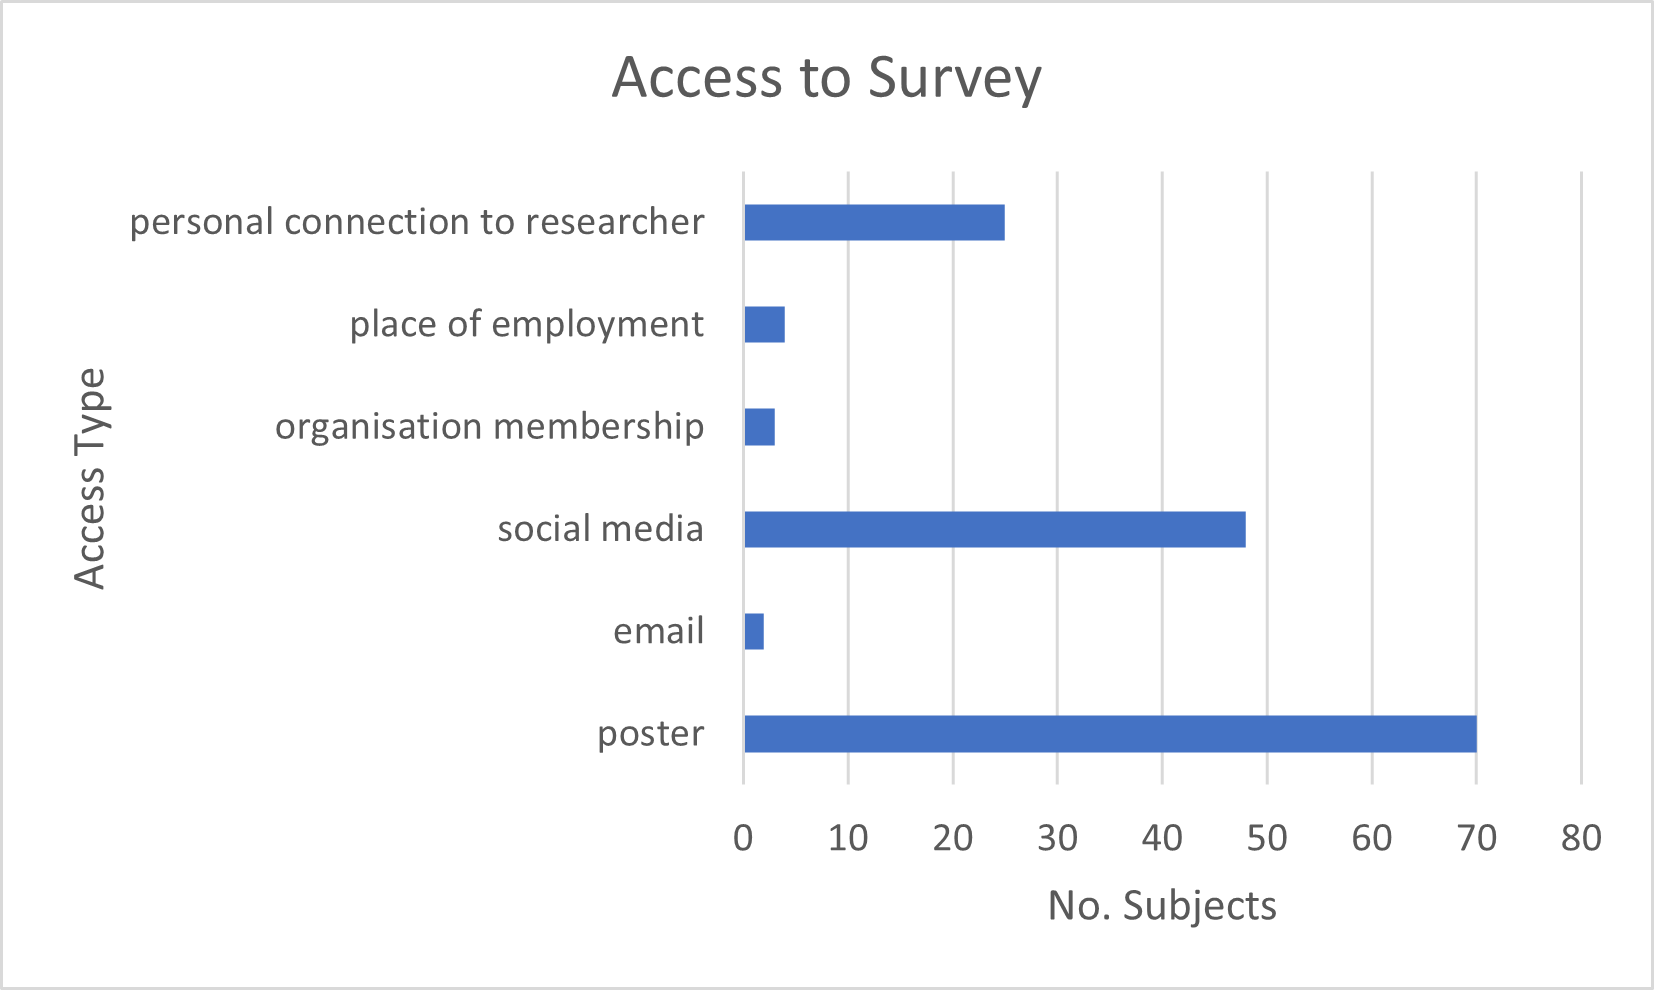
\includegraphics{fig_results/access_survey.png}
    \caption{Access to Survey}. The most common access method of the survey was poster, with 70 subjects selecting this choice. This is followed by social media which has 47 subjects choosing this. Only 25 subjects accessed the survey due to personal connection to researcher. Access via email, place of employment and organisation membership are all under 10. Subjects could chose more than one access type. For example a subject could have accessed via personal connection to researcher and social media, due to the researcher sharing this survey on her personal page.
    \label{fig:my_label}
\end{figure}
\paragraph{}

\subsection{Perceived Risks}

\begin{figure}[h]
    \centering
    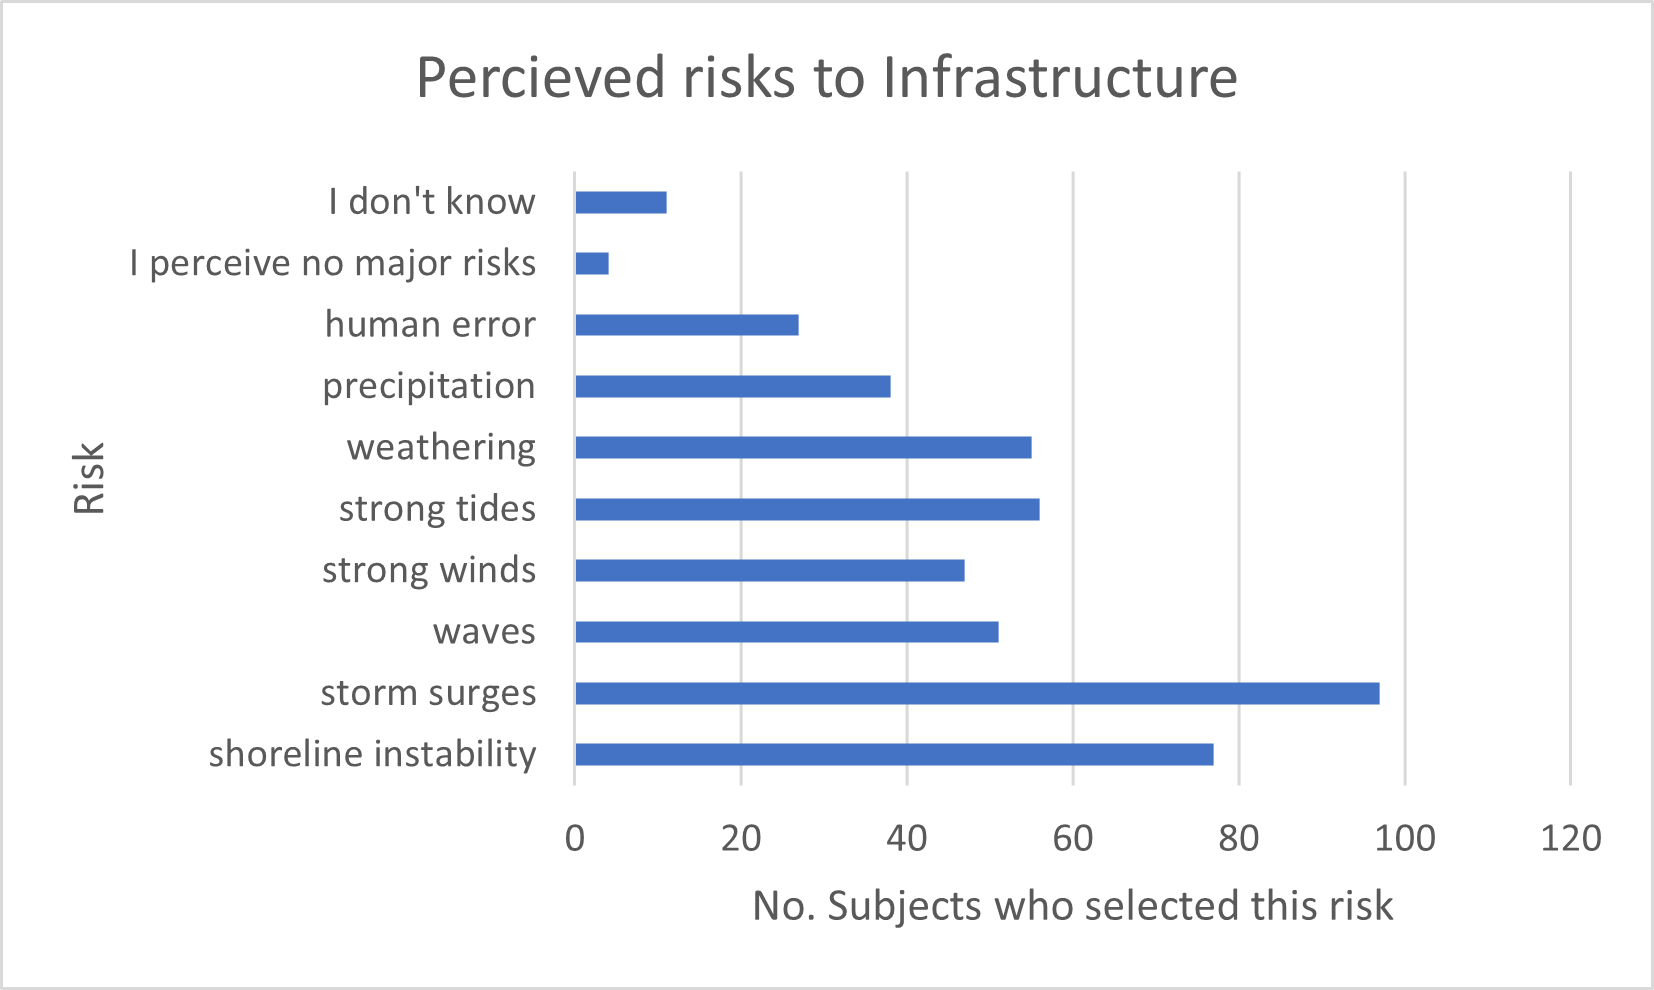
\includegraphics{fig_results/infrastructure-risks.png}
    \caption{Infrastructure Risks}
    \label{fig:my_label}
\end{figure}
\paragraph{}
words words words

\begin{figure}[h]
    \centering
    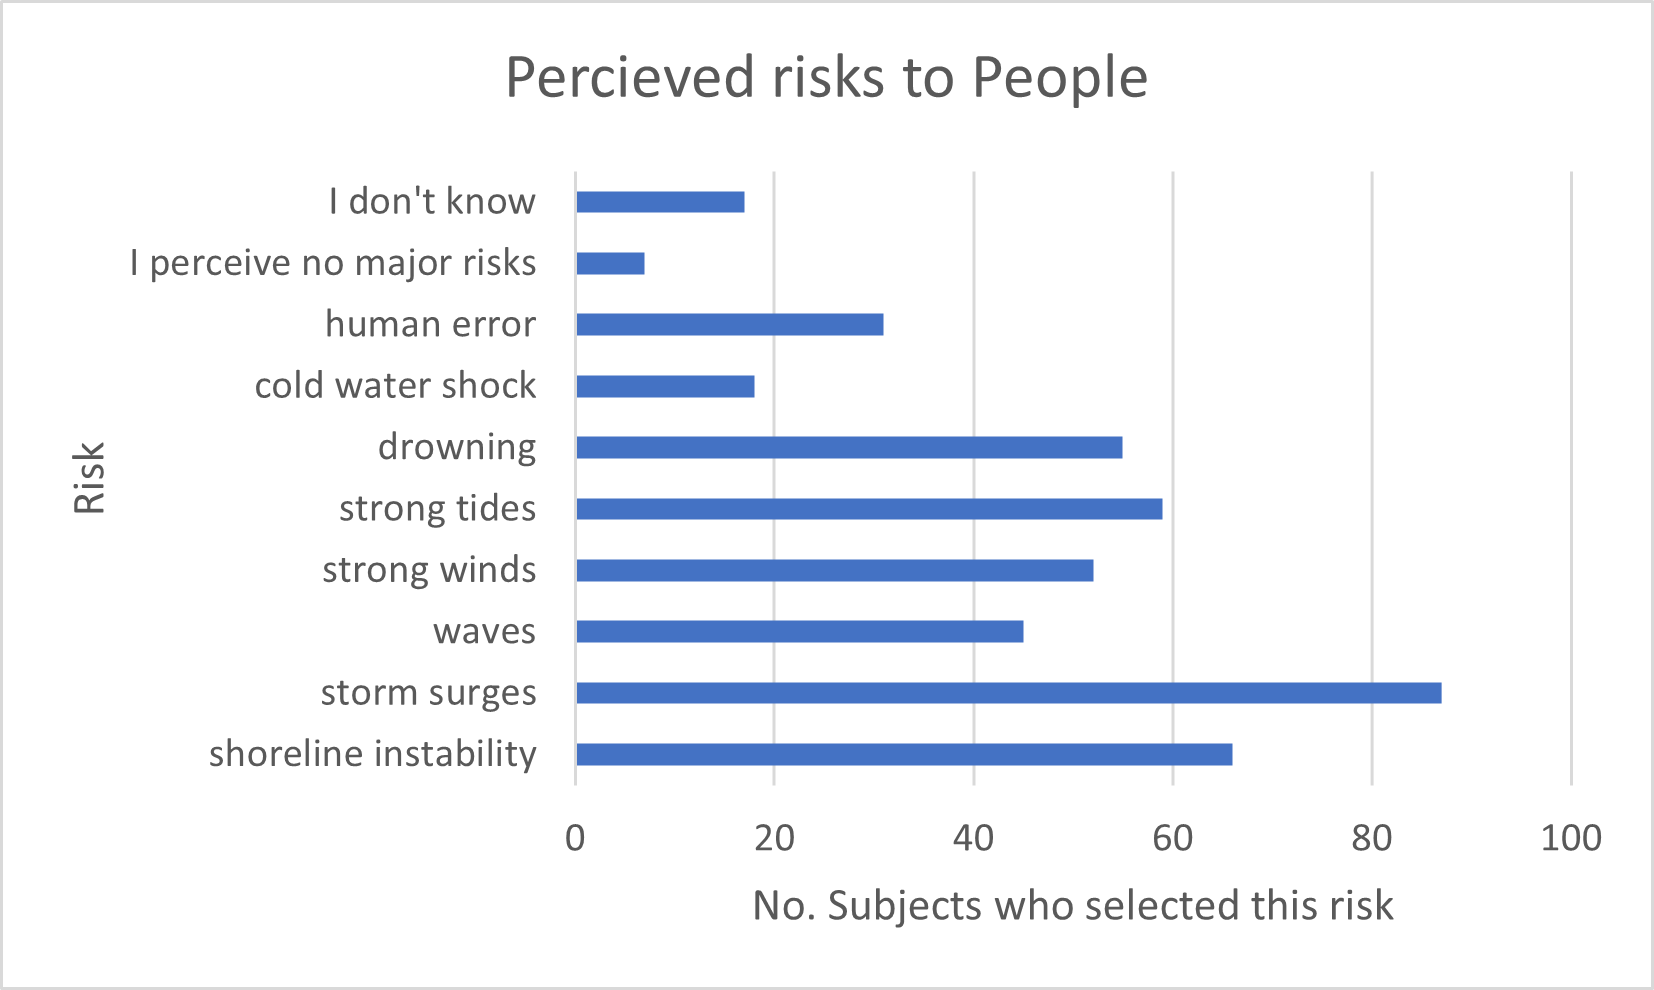
\includegraphics{fig_results/people-risks.png}
    \caption{People risks}
    \label{fig:my_label}
\end{figure}
\paragraph{}

\section{Awareness}

\begin{figure}[h]
    \centering
    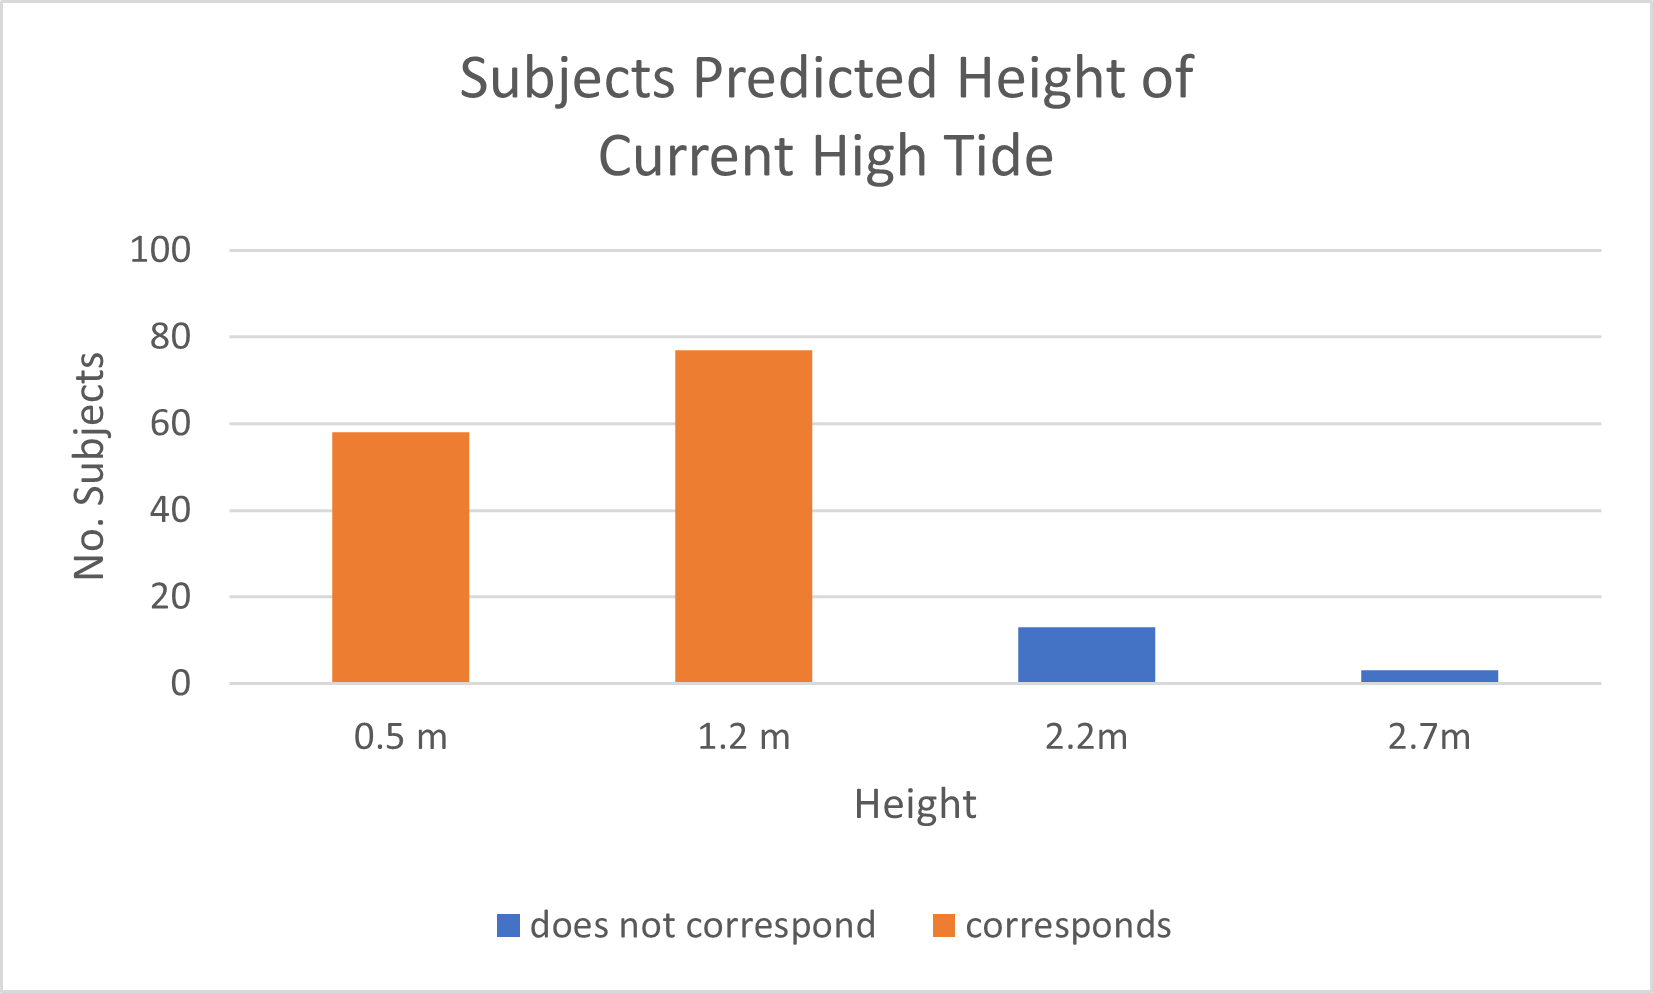
\includegraphics{fig_results/2022-hightide-answers.png}
    \caption{Subjects Predicted Height of Current High Tide. Height 0.5m is the neep high tide, Height 1.2m is the Spring High Tide. Th vast majority of subjects got an answer which corresponds with models of tides in Trondheim. Under 20 subjects responded with an answer which does not correspond with models of tides. 58 subjects chose 0.5m, 77 subjects chose 1.2m meaning that 135 out of 153 subjects, 88 percent chose what could be considered the correct answer for high tide. While only 13 subjects chose 2.2m and 3 subjects chose 2.7m}
    \label{fig:high-tide-answer}
\end{figure}
\paragraph{}
As can be seen in figure ** above the subjects displayed a high awareness of the tides in Trondheim. Under 20 subjects responded with an answer which does not reflect the models from \cite{kartverket_se_2021}. Over 88 percent of subjects chose a value which matches with models by \cite{kartverket_se_2021} The majority of respondents chose the answer of 1.2m which corresponds with the Spring tide. 

\begin{figure}[h]
    \centering
    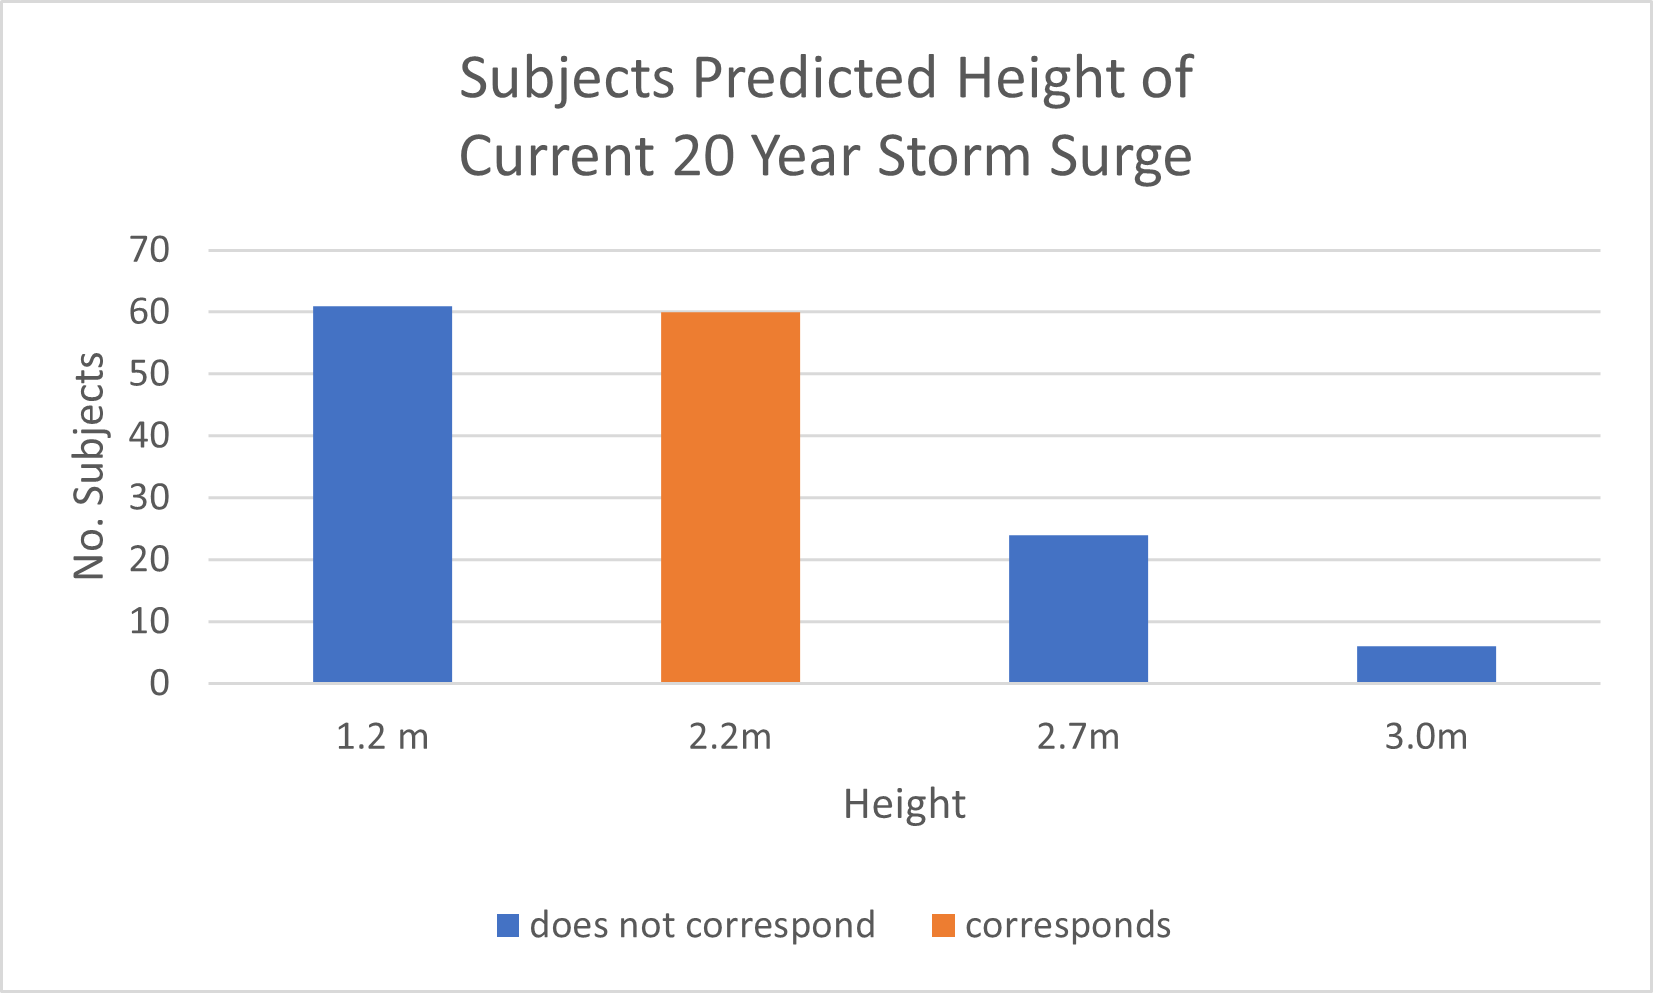
\includegraphics{fig_results/2022-20yrss-answer.png}
    \caption{Subjects Predicted Height of Current 20 Year Storm Surge. 61 subjects chose 1.2m this is very comparable to the 60 which chose 2.2m which is the answer which corresponds with \cite{kartverket_se_2021}. 24 subjects chose 2.7m and only 6 subjectts chose 3.0m}
    \label{fig:2022-stormsurge-answers}
\end{figure}
\paragraph{}
The majority of subjects chose 1.2m as the predicted height of the 20 year storm surge, this does not correspond with models from \cite{kartverket_se_2021}. In fact 1.2m is equal to the current high tide. Almost equally well chosen was the answer which does correspond with models from \cite{kartverket_se_2021}, 2.2m, with 60 subjects choosing this answer. This means that 43 percent of subjects chose the answer which corresponds with \cite{kartverket_se_2021}.

\begin{figure}[h]
    \centering
    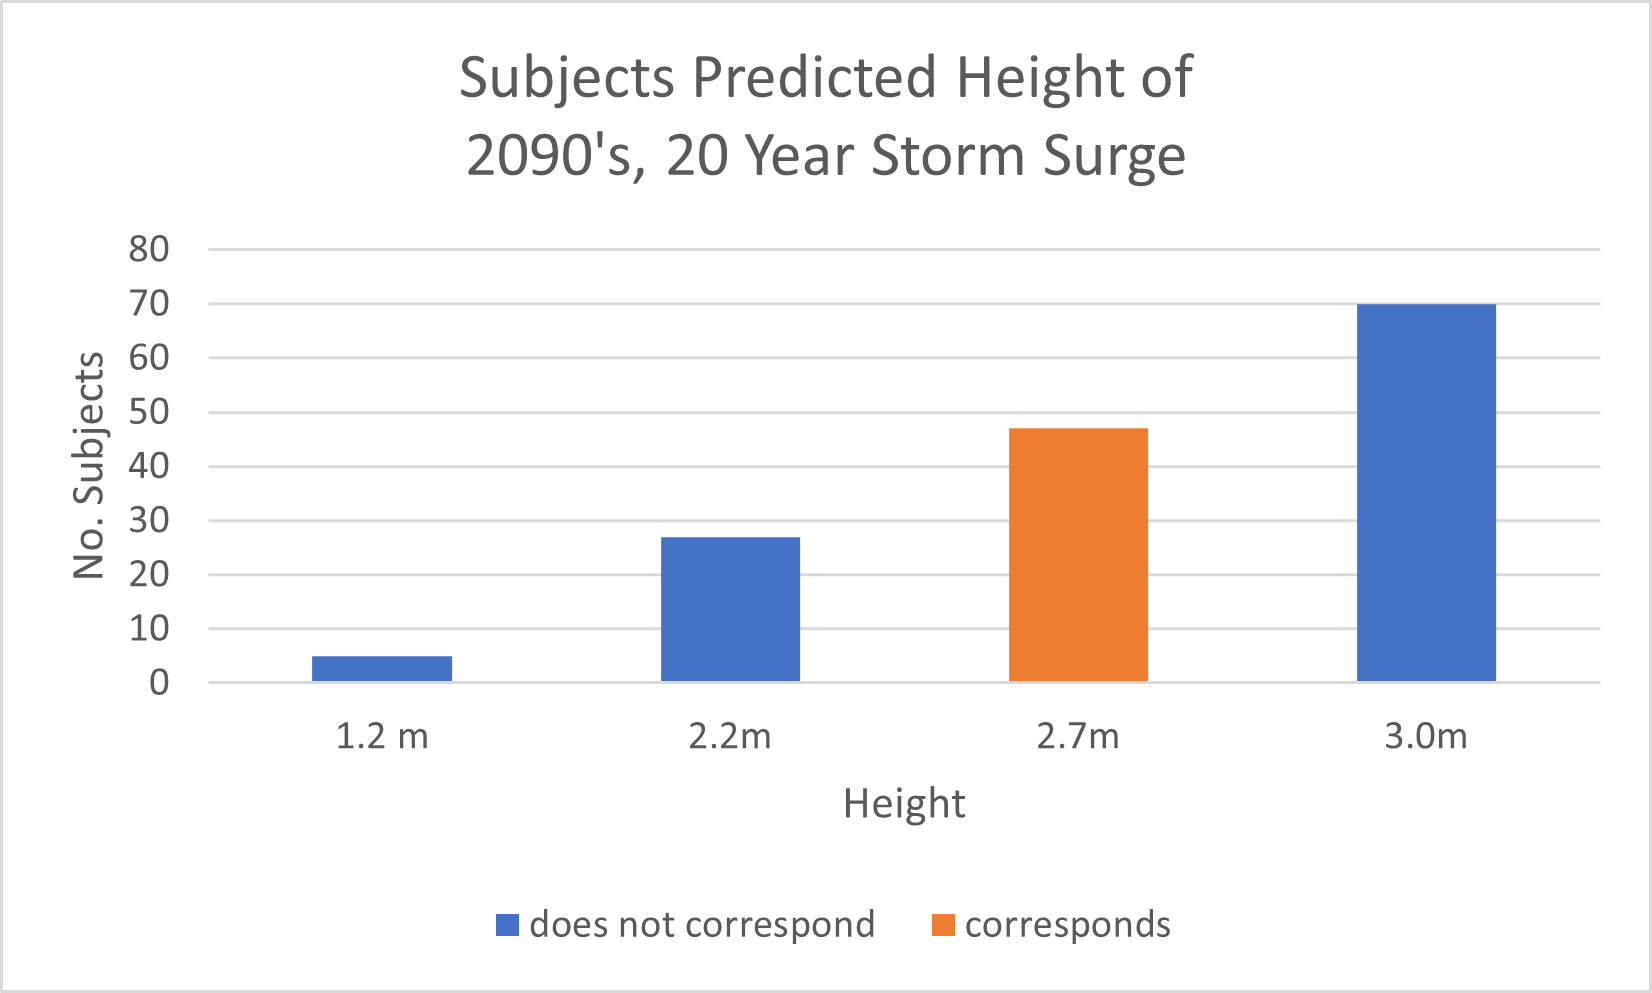
\includegraphics{fig_results/2090s 20yr ss answers.png}
    \caption{Subjects Predicted Height of 2090's, 20 year storm surge. The majority of subjects chose the highest value with 70 subjects choosing 3.0m as the predicted height of the storm surge. 47 subjects chose 2.7m which is the value which corresponds with models by \cite{kartverket_se_2021}. 27 subjects chose 2.2m and only 5 subjects chose 1.2m}
    \label{fig:2090-stormsurge-answers}
\end{figure}
\paragraph{}
The majority of subjects predicted the storm surge in 2090 to be 3.0m. Just over 30 percent chose 2.7m which is the value which corresponds with models from \cite{kartverket_se_2021}. This means that most people thought the sea level extreme associated with the 20 year storm surge in 2090 is higher than it is currently predicted to be. The change of height for the 20 year storm surge predicted for 2090 is only 50cm higher than the current 20 year storm surge \cite{kartverket_se_2021}. 
\paragraph{}

\begin{figure}[h]
    \centering
    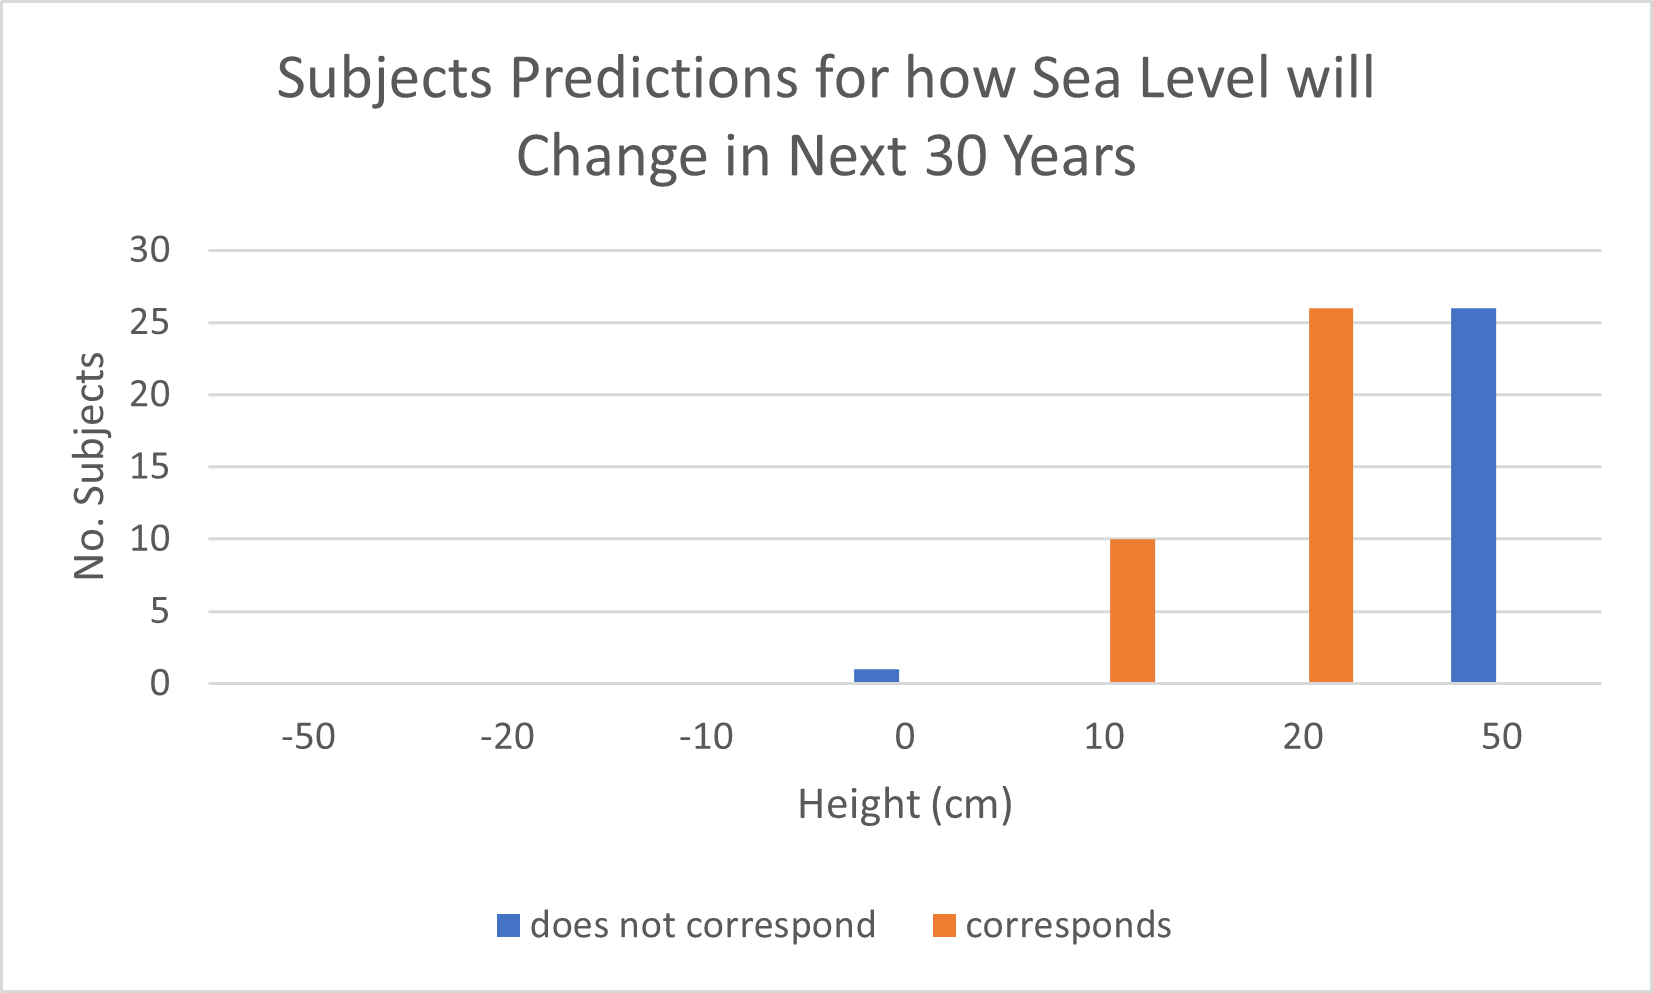
\includegraphics{fig_results/slr-future.png}
    \caption{Subjects Predictions for how Sea Level will change in Trondheim in Next 30 years. Only 147 subjects answered for this question, unlike every other one which all subjects, 153, answered. No subjects believed the sea level will decrease over the next 30 years. One subject answered that it will stay the same, with every other subject chosing that it will rise by some level }
    \label{fig:my_label}
\end{figure}

There is strong uncertainty with this measurement in models, due to the unknown of emisson patterns over the next 30 years and isostatic uplift. Never the less an estimation of 20cm or 10cm is in line with \cite{kartverket_se_2021} which uses the upper emissions pathways from the IPCC. Over half of subjects chose an answer which is in line with models from \cite{kartverket_se_2021}. However equal numbers of subjects,26, chose 50cm which is not in line with these models as chose 20cm. Almost all subjects answered that sea level will rise in the next 30 years, though six subjects chose not to answer this question.  

\begin{figure}[h]
    \centering
    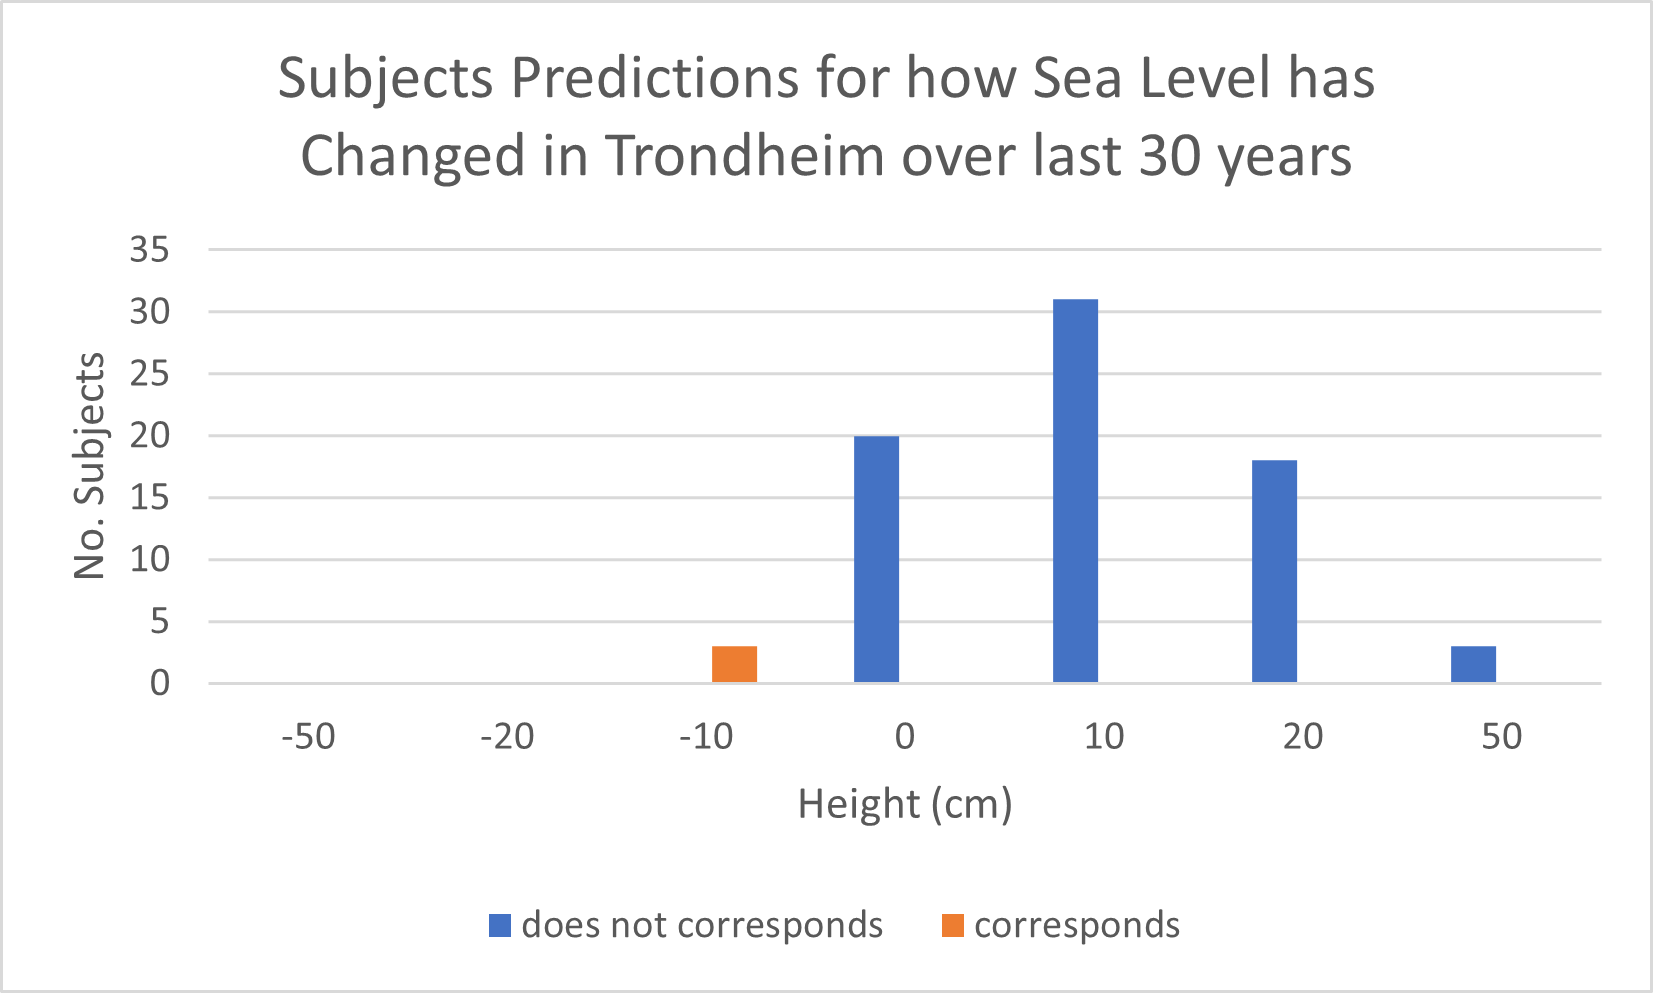
\includegraphics{fig_results/slr-past.png}
    \caption{Subjects Predictions for how Sea Level has Changed in Trondheim over last 30 years. Only 3 subjects chose that sea level has decreased in the last 30 years, this answer is inline with \cite{kartverket_se_2021}. 20 subjects answered that sea level had not changed over this time. While 31 subjects answered that it had risen by 10 cm. 18 subjects answered that it had risen by 20 cm and 3 answered that it had risen by 50 cm. 52 subjects answered that sea level had risen over the last 30 years. }
    \label{fig:my_label}
\end{figure}

The next figure also 
\begin{figure}[h]
    \centering
    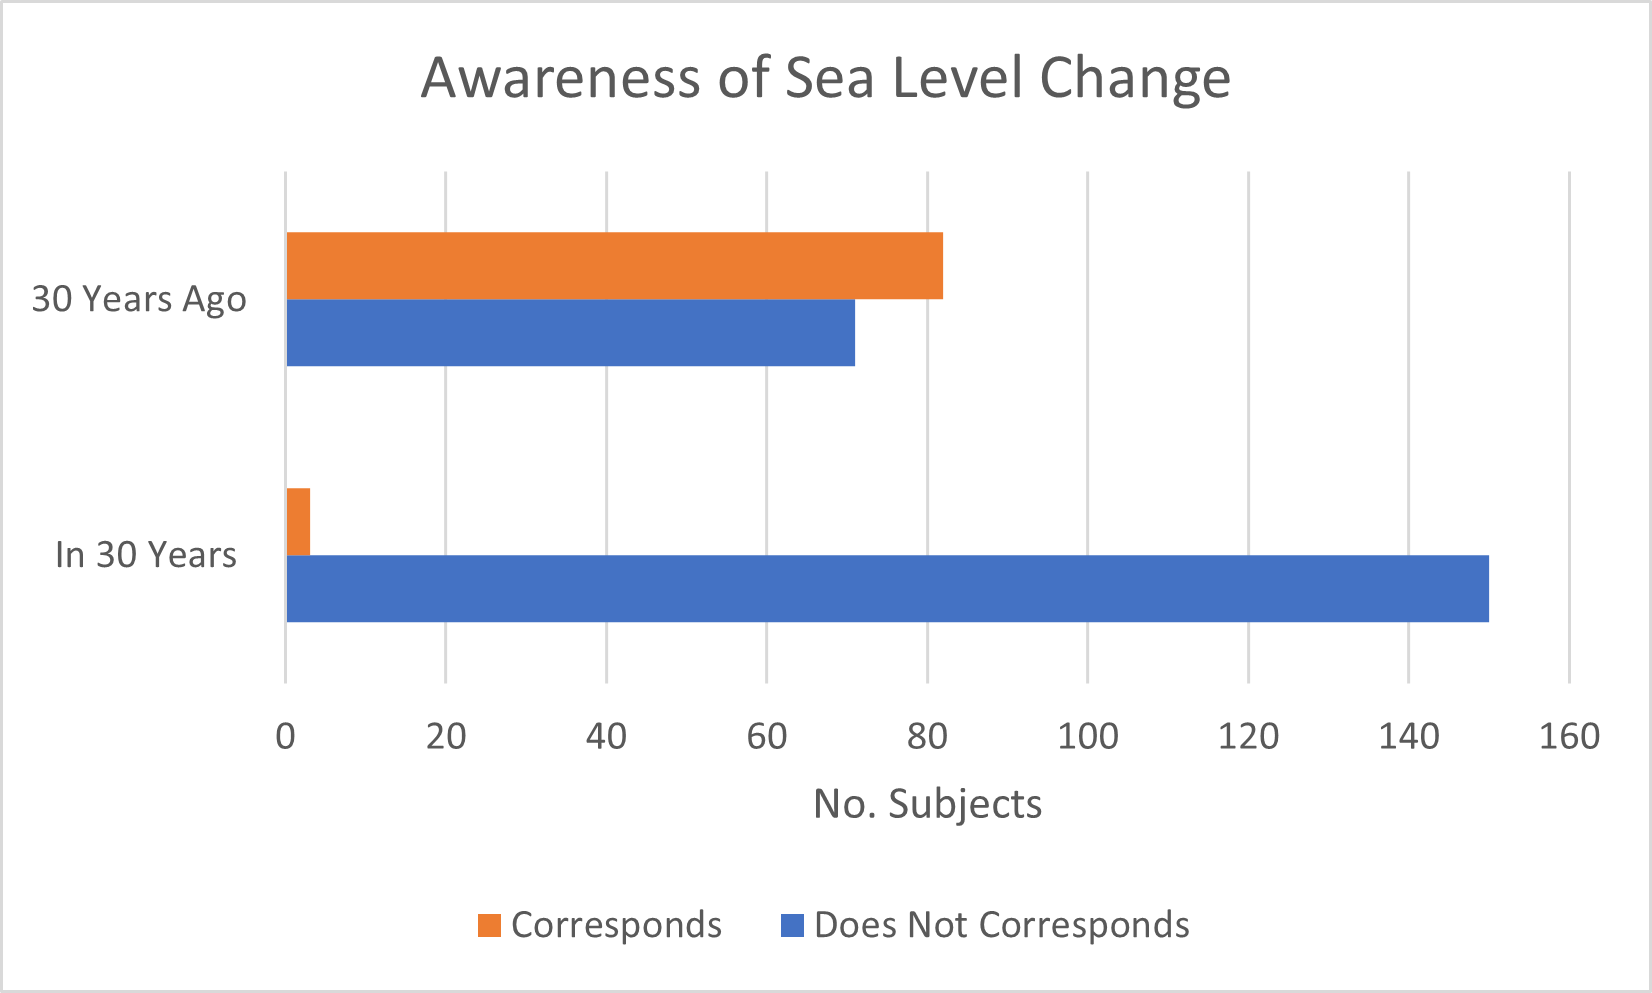
\includegraphics{fig_results/Aware_sea_level_change.png}
    \caption{Awareness of Sea Level Change. Only 3 subjects chose an answer which corresponds with the models from \cite{kartverket_se_2021}, for what height sea level in Trondheim will be in 20 years time. In contrast 82 subjects just over half chose an answer which corresponds with models from \cite{kartverket_se_2021} for what the sea level was 30 years ago. }
    \label{fig:my_label}
\end{figure}
\paragraph{}

For both of these questions 

Figure.... below is the sum of all results pictured above in this section on awareness. This was the first attempt to determine awareness of subjects from the results of this survey

\begin{figure}[h]
    \centering
    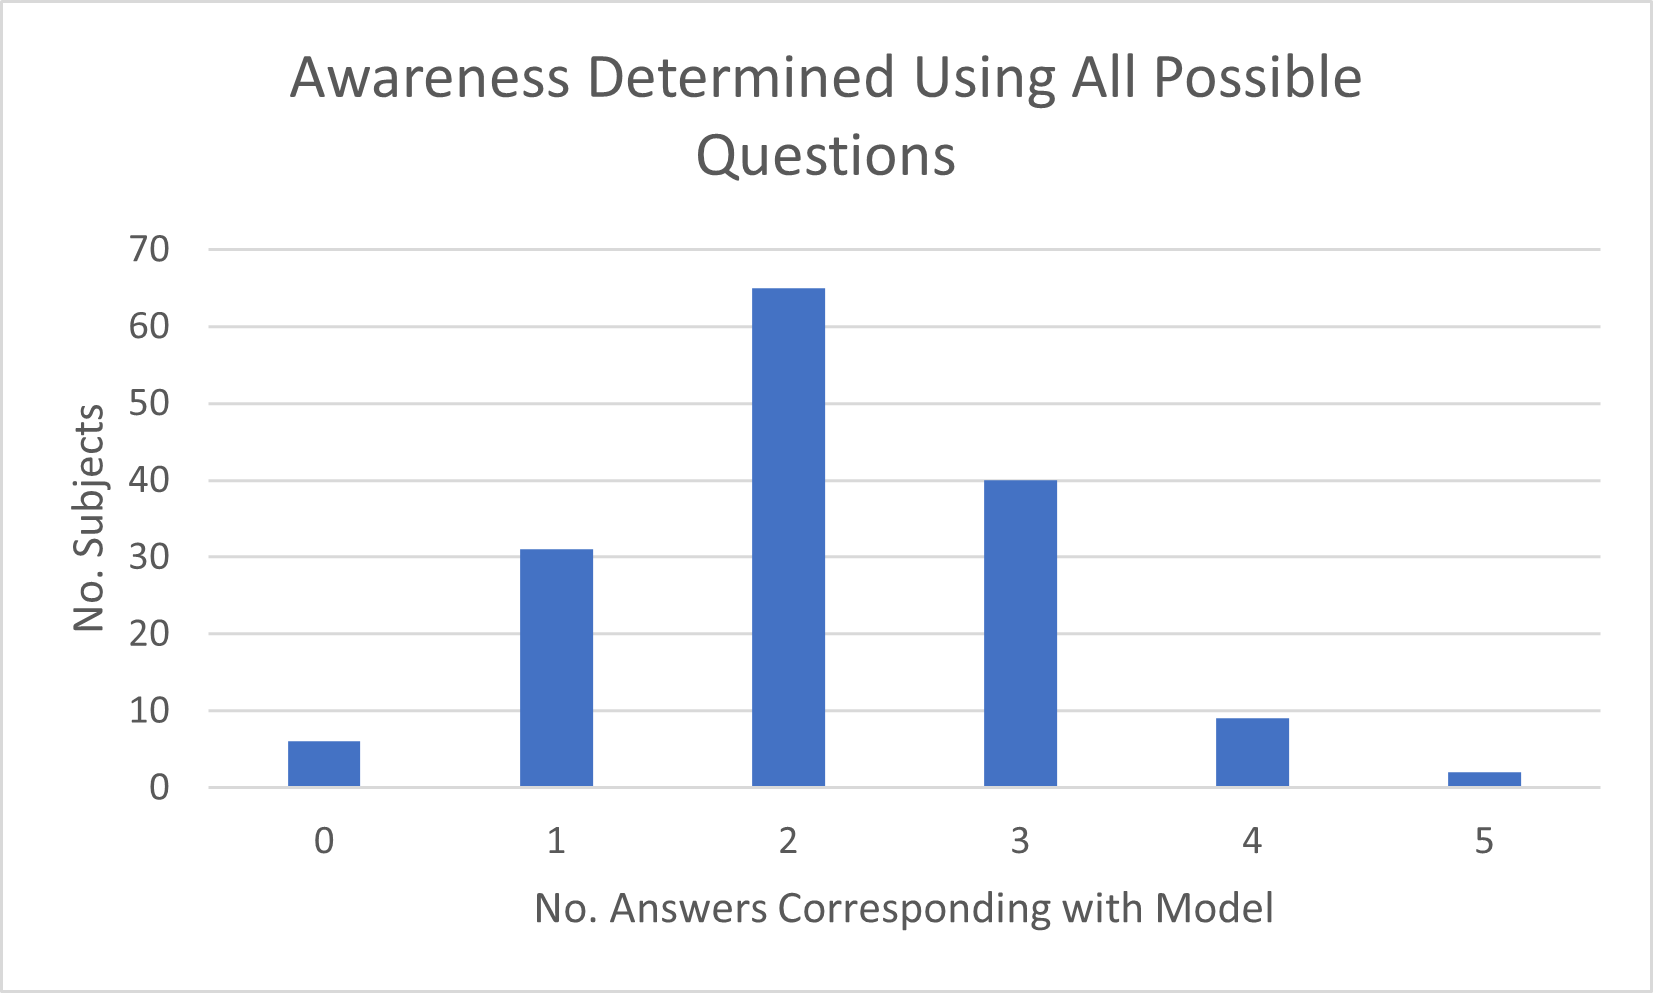
\includegraphics{fig_results/aware_all.png}
    \caption{Awareness Considering all Questions which were designed to determine awareness}
    \label{fig:aware-all}
\end{figure}
\paragraph{}

Due to the reasons expanded upon in the discussion of results, awareness determination considering all answers related to questions was not the most suitable for analysing factors related to awareness. For this reason another determination of awareness was created utilising only the questions which had pictures of the simulated water levels. 

\begin{figure}[h]
    \centering
    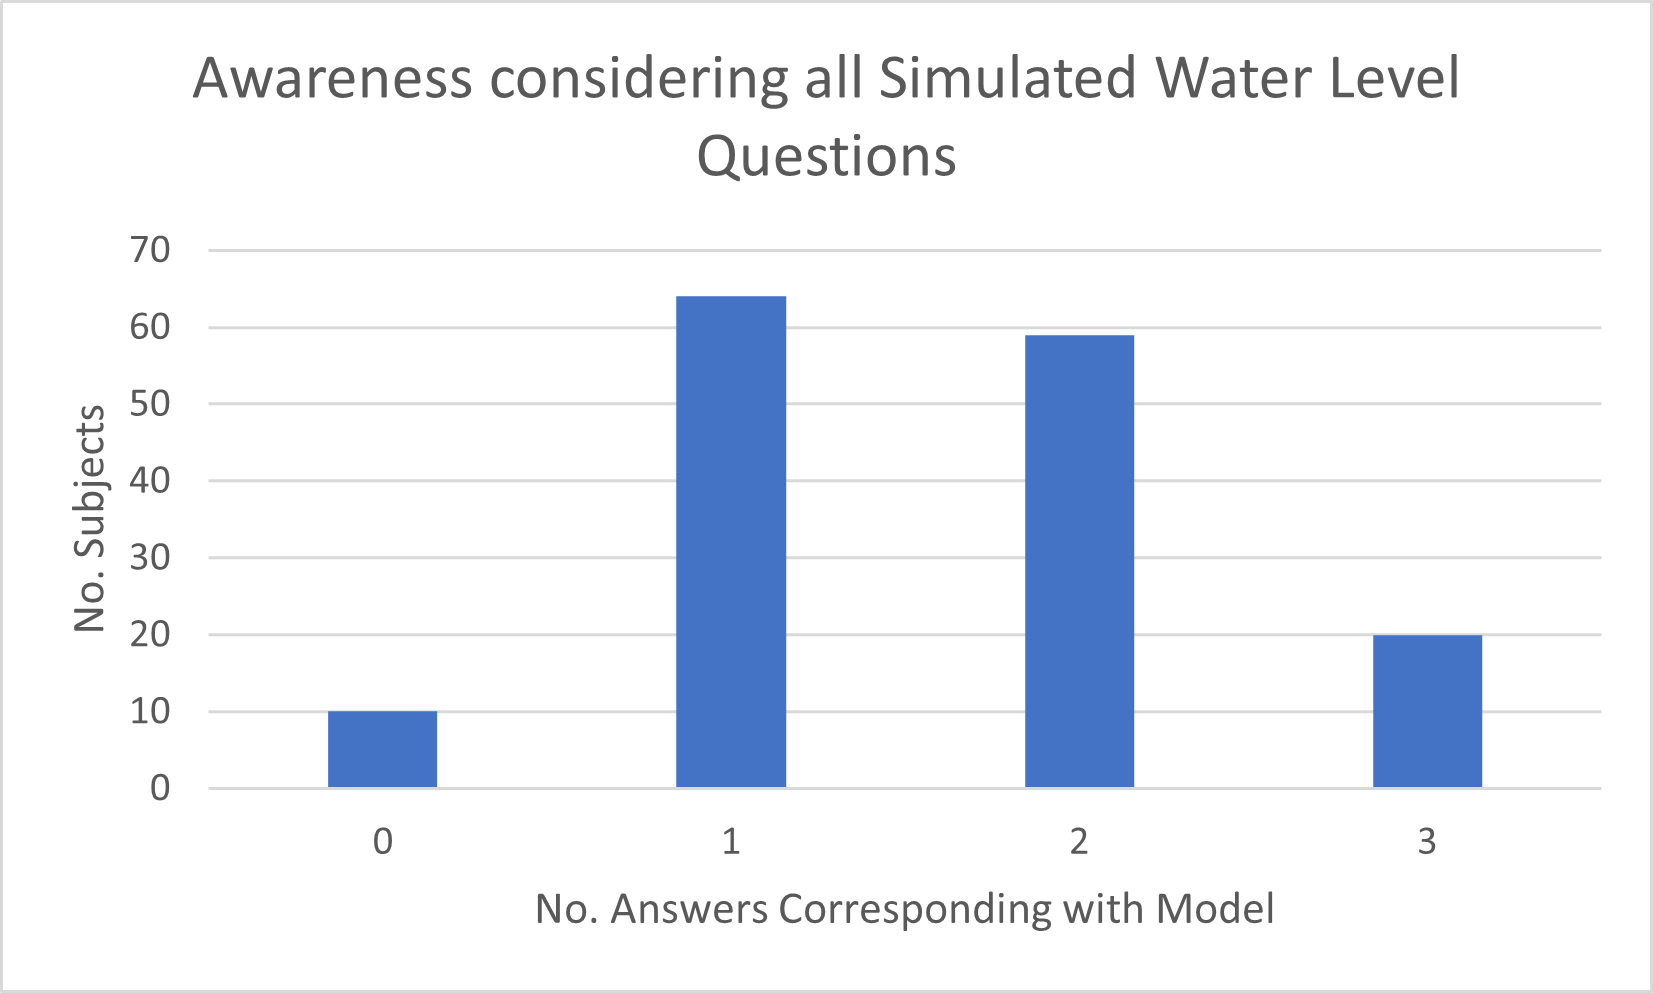
\includegraphics{fig_results/Awareness_ all_simulation_pictures_qs.png}
    \caption{Awareness considering all Simulated Water Level Questions}
    \label{fig:aware_all}
\end{figure}

The determination of awareness displayed in the figure above was chosen as the most appropriate variable due to the fact that only awareness questions with a simulated water level picture were included, as can be seen in the appendix. The other determination of awareness included the results from two questions which are based purely off numeric answers which gave very skewed results. When given just numeric responses the accurate rate was non significant. For example only 3 subjects out of 153 gave the correct answer for slr-past, which is very unlikely given that it was multiple choice with only 7 potential answers (if split evenly then would have 21 subjects choosing this response. While slr-future had more correct responses, this was only mildly significant which combined the lack of correct answers for slr-past was seen as a good reason to exclude the answers to both of these questions for creating the variable of awareness. 

Another determination of awareness was considered which only includes results from questions on current storm surge and current high tide, excluding results of the question of the 20 year storm surge in 2090. This was considered as a potential baseline variable for current awareness to sea level extremes as different from awareness to future sea levl extremes. However the variable summary statistics are incredibly similar. 




\paragraph{}
As shown by the focus group there is issues with just requesting a numeric value from subjects. There is a higher potential connection for many individuals including another emotional layer when using pictures rather than numbers. 

\section{Factors Affecting Awareness}
The results from the survey for both the variables and factors were very skewed as can be seen from the figures above. The analysis was first done on R and then exported to excel to utilise their templates for graphs. The results from the histogram analysis is that no variable of awareness appeared normally distributed. Upon basic transformation including logarithmic and cubing it was highly skewed. Further more almost all factors from the results were skewed as can be seen in the figures above.   

\subsection{Shapiro Test Results}

During histogram analysis only the factors of "interest-level" and "info-sum-climate" appeared normally distributed. To investigate whether these variables were truly normally distributed a Shapiro test was carried out using \cite{royston_extension_1982} . Due to inexperience with this method it was first checked on variables which from the histograms were clearly skewed. From these tests and \cite{royston_extension_1982} an assumption of alpha value of 0.05 was determined meaningful. This means if the p-value created during this test is below 0.05 then the null hypothesis is rejected. This does leave a 5 percent chance of error. The results from the Shapiro test can be seen in table* below and this determines that none of the variables were normally distributed. 

\begin{table}[h]
    \centering
    \begin{tabular}{|l|l|l|l|}
    \hline
         Variable & W-value & P-Value & Distribution \\ \hline
       Interest Level & 0.89332 & 4.343e-09 & Skewed \\ \hline
         Info Climate Sum  & 0.95721 & 0.0001159 & Skewed \\ \hline
        Flood Impact & 0.87779 & 6.681e-10 & Skewed \\ \hline
     \end{tabular}
    \caption{Shapiro Test Results. The alpha value was assigned 0.05, meaning that if the p-value is below 0.05 then the null hypothesis that this factor is not normally distributed was rejected. This leaves a 5 percent chance of error. Each of these factors p-value is below 0.05 meaning that their distribution was deemed skewed.}
    \label{table:shapiro_test_results}
\end{table}
\paragraph{}

This result that all variables and factors were skewed including the important variable of awareness and interest level influenced the choice of how to analyse dependency. Mixed effect linear models were considered, but the purpose of this project was to find fast ways of analysing resilience and what social factors could be worked on to improve resilience. For this reason non-parametric tests was decided upon. Kruskal Wallis Rank Sum Tests were chosen due to the need to investigate multiple groups, upon one factor -awareness- and having only measured each subject once. Both \cite{tasman_how_2014} and \cite{hollander_nonparametric_2014} were consulted to make this decision. 

\subsection{Kruskal Wallis Rank Sum Test}
Kruskal Wallis Rank Sum Test was conducted using R, specifically the package based off \cite{hollander_nonparametric_2014}. Kruskal Wallis Rank Sum Test was chosen due to the the distribution of the results and the potential inter-dependency of the data. Linear modelling was also considered and trialled, but this technique includes the skewed aspect of the data better, when looking for dependents. An alpha value of 0.05 was chosen before these test were carried out. This means there is a 5 percent chance of inaccuracy when determining dependency of factors against the variable of awareness.

\begin{table}[h]
    \centering
    \begin{tabular}{|l|l|l|l|}
    \hline
         ~ &Awareness as predictor & ~ & ~ \\ \hline
        Factor & p value & h value & df \\ \hline
           length of Knowledge & 0.73760 & 3.54770 & 6 \\ \hline
       Interest Level in SLE & 0.16920 & 6.43150 & 4 \\ \hline
        Concern about Climate & \cellcolor[HTML]{7df9ff} 0.05630 & 9.19960 & 4 \\ \hline
        Language of Survey & 0.2041 & 1.6129 & 1 \\ \hline
        Predicted Personal Impact of Flood & 0.7156 & 1.357 & 3 \\ \hline
    \end{tabular}
    \caption{Kruskal Wallis Test Results General Variables}
    \label{Kruskal_wallis_test_general}
\end{table}

In this case none of the factors were deemed significant as all the p-values were larger than the alpha value of 0.05. However the factor of Concern about climate change is 0.05630, which is very near. If the alpha value was chosen to be 0.01 as is used in some studies \cite{hollander_nonparametric_2014} then this would be enough to reject the null hypothesis that concern about awareness is not dependent upon concern about climate. Another way the hypothesis could have been accepted is due to the high h-value, however as df was under 5 this did not give enough confidence to accept the hypothesis \cite{minitab_interpret_2022}. The conclusion here is that there is not strong enough evidence that awareness is dependent upon Concern about Climate.




\begin{table}[h]
    \centering
    \begin{tabular}{|l|l|l|l|}
    \hline
         ~ &Awareness as predictor & ~ & ~ \\ \hline
        Factor & p value & h value & df \\ \hline
        Sum & 0.52060 & 4.20260 & 1 \\ \hline
        Marine worker & na & na & na \\ \hline
        Worker & 0.12310 & 2.37220 & 1 \\ \hline
        Resident & \cellcolor[HTML]{7df9ff} 0.01524 & 5.88900 & 1 \\ \hline
        Student & 0.55590 & 0.34691 & 1 \\ \hline
        Leisure User Land & 0.68790 & 0.16141 & 1 \\ \hline
        Leisure User water & 0.42120 & 0.64690 & 1 \\ \hline
        Commuter & 0.44610 & 0.58063 & 1 \\ \hline
        Other & 0.58620 & 0.29627 & 1 \\ \hline
    \end{tabular}
    \caption{Kruskal Wallis Test Results Community Membership. Other community membership was self reporting the most common response was tourist, with sailor coming next. Resident is the only value which is highlighted here as it was the only significant result when utilising a alhpa value of 0.05}
    \label{Kruskal_wallis_test_general}
\end{table}

An alpha value of 0.05 was chosen and the factor of community membership - resident has a P-value of 0.01524, hence is significant. Meaning the null hypothesis of no relationship was rejected and the positive hypothesis that residency is dependent on awareness was accepted. 




As the P-value for the variable community membership -residence is greater than the alpha (could assign 0.05 as is common or assign 0.1 which would make it easier to include a few more variables for discussion) The differences between some of the medians are statistically significant.

\begin{table}[h]
    \centering
    \begin{tabular}{|l|l|l|l|l|l|l|}
    \hline
        variable name & p value & h value & df & p value & h value & df \\ \hline
        predictor & ss\_aware & ~ & ~ & ss\_aware\_2 & ~ & ~ \\ \hline
        info\_place\_sum & 0.44600 & 6.85110 & 7 & 0.45040 & 6.79650 & 7 \\ \hline
        info\_place\_po & 0.22730 & 1.45790 & 1 & 0.36470 & 0.82162 & 1 \\ \hline
        info\_place\_family & 0.78550 & 0.07406 & 1 & 0.81340 & 0.05572 & 1 \\ \hline
        info\_place\_friend & 0.27580 & 1.18780 & 1 & 0.30200 & 1.06520 & 1 \\ \hline
        info\_place\_newspaper & 0.74490 & 0.10583 & 1 & 0.48500 & 0.48765 & 1 \\ \hline
        info\_place\_tv & 0.87330 & 0.02542 & 1 & 0.33420 & 0.93237 & 1 \\ \hline
        info\_place\_so\_me & 0.48540 & 0.48671 & 1 & 0.95090 & 0.00379 & 1 \\ \hline
        info\_place\_mem & 0.67530 & 0.17550 & 1 & 0.70980 & 0.13848 & 1 \\ \hline
        info\_place\_kommune & 0.82590 & 0.04839 & 1 & 0.12790 & 0.57600 & 1 \\ \hline
        info\_climate\_sum & 0.91220 & 3.32660 & 8 & 0.45218 & 8.12040 & 8 \\ \hline
        info\_climate\_po & 0.11750 & 2.45020 & 1 & 0.24550 & 1.34870 & 1 \\ \hline
        info\_climate\_family & \cellcolor[HTML]{7df9ff} 0.00481 & 0.94470 & 1 & 0.56970 & 0.32313 & 1 \\ \hline
        info\_climate\_friend & 0.82460 & 0.04910 & 1 & 0.63010 & 0.23186 & 1 \\ \hline
        info\_climate\_newspaper & 0.09036 & 2.86790 & 1 & \cellcolor[HTML]{7df9ff} 0.01218 & 6.24830 & 1 \\ \hline
        info\_climate\_tv & 0.61230 & 0.25689 & 1 & 0.75000 & 0.10154 & 1 \\ \hline
        info\_climate\_so\_me & 0.74950 & 0.10960 & 1 & 0.92830 & 0.00809 & 1 \\ \hline
        info\_climate\_mem & 0.30270 & 1.06220 & 1 & 0.27500 & 1.91500 & 1 \\ \hline
        info\_climate\_sci & 0.88040 & 0.02650 & 1 & 0.12390 & 2.36760 & 1 \\ \hline
        info\_climate\_edu & 0.64850 & 0.20779 & 1 & \cellcolor[HTML]{7df9ff} 0.02438 & 5.06770 & 1 \\ \hline
    \end{tabular}
    \caption{Kruskal Wallis Test Results Variables on Information Access}
    \label{Kruskal_wallis_test_information}
\end{table}

Kruskal wallis test indicate that com-mem-resident is a factor for ss-aware, it could be a random factor, which would mean a more appropriate method than basic linear modelling is linear mixed effect modelling. Linear mixed effect modelling should consider com-resident as a random factor for ss-aware and for ss-aware-2, then infor-climate-edu and info-climate-newspaper may be random factors.

Info-climate-sum and com-mem included factors which influence the chosen baseline variable, but do not in and of themselves appear dependent from the kruskal wallis test. However it does highlight that these factors may be important considerations and are worth trialling with linear mixed effect modeeling.



\section{Hypothesis Testing Summary}
To summarise the results from the hypothesis testing it is put in the format of the original hypothesises shown in the introduction. 
%could break it down into section is 
%\subsection{ Awareness and Place}
%\subsection{Awareness and Language}
%\subsection{Awareness and Community Membership}
%\subsection{Awareness and Level of Interest}
%\subsection{Awareness and Information Access}

\subsection{Hypothesis dependent on community membership}
\begin{enumerate}
    \item We expect residents to be aware - accepted
    \item We expect commuters to be aware - rejected
    \item We expect marine workers to be aware - no result
    \item We expect non-marine workers to be unaware - no result
    \item We expect water leisure users to be aware - rejected
    \item We expect land leisure users to be unaware - rejected
    \end{enumerate}
\paragraph{}

\subsection{Hypothesis dependent on local knowledge}
\begin{enumerate}
    \item We expect subjects with professional interest in SLE's to be aware - not accepted
    \item We expect subjects with primary knowledge about places which are on reclaimed land to be aware
    \item We expect subjects with a length of knowledge greater than 20 years of the area to be aware -  awareness does not appear to be dependent on length of knowledge
    \item We expect subjects with a length of knowledge less than 1 year of the area to be aware -   awareness does not appear to be dependent on length of knowledge
    \item We expect subjects with many information sources about the place to be more aware - awareness does not appear to be dependent on information sources about place
    \item We expect subjects who chose to respond in Norwegian to be aware - no observation of awareness being dependent on whether the subjects responded in Norwegian or English
\end{enumerate}
\paragraph{}

\subsection{Hypothesis dependent on awareness of changing climate}
\begin{enumerate}
    \item We expect subjects with many information sources about climate change to be more aware - awareness does appear to have a dependency on where the subject got information about the climate from, however there is no observed link between more sources having a greater impact on awareness
    \item We expect subjects with the information source of formal education and/or peer reviewed publications to be aware - awareness does not have an observed dependency on subjects getting information from peer review publications. Awareness of the current sea level extremes, but not the future ones does appear to be dependent upon getting information about the climate from formal education.  
    \item We expect subjects who are more concerned about climate change to be aware - it is not particularly significant but we have found that awareness is not dependent upon climate change, but further research is needed on this result as it was borderline and could have been shifted in a slightly larger alpha value was chosen.
    \item We expect subjects who predict they will be impacted by flooding from SLE's to be more aware - hypothesis rejected
\end{enumerate}

Very few of the hypothesis were accepted. The reasons for this are expanded upon in the next section Discussion of Results